\documentclass[12pt,a4paper]{article}

\usepackage[indonesian]{babel}
\usepackage{fontspec}
\setmainfont{Times New Roman}
\setsansfont{Arial}
\setmonofont{Consolas}[Scale=0.88]

\usepackage[top=3cm,bottom=2.5cm,left=3.5cm,right=2.5cm,headheight=15pt]{geometry}
\usepackage{graphicx}
\usepackage{xcolor}
\usepackage{titlesec}
\usepackage{fancyhdr}
\usepackage{lastpage}
\usepackage{booktabs}
\usepackage{tabularx}
\usepackage{longtable}
\usepackage{array}
\usepackage{colortbl}
\usepackage{multirow}
\usepackage{enumitem}
\usepackage{setspace}
\usepackage{parskip}
\usepackage{needspace}
\usepackage{tocloft}
\usepackage{tikz}
\usetikzlibrary{arrows.meta,positioning,shapes.geometric,fit,backgrounds}
\usepackage{listings}
\usepackage{hyperref}

\definecolor{PolibatamBlue}{HTML}{2F5496}
\definecolor{TableHeadBg}{HTML}{E8EEF6}
\definecolor{RowShade}{HTML}{F5F7FA}
\definecolor{JajanGreen}{HTML}{2E8B3D}
\definecolor{ActorFill}{HTML}{F0F6FC}

\renewcommand{\lstlistingname}{Kode}
\lstset{
  basicstyle=\ttfamily\fontsize{9}{11}\selectfont,
  backgroundcolor=\color{RowShade},
  frame=single,
  rulecolor=\color{PolibatamBlue},
  breaklines=true,
  columns=fullflexible,
  keepspaces=true,
  showstringspaces=false,
  commentstyle=\color{JajanGreen}\itshape,
  keywordstyle=\color{PolibatamBlue}\bfseries,
  stringstyle=\color{black!75}
}

\hypersetup{
  colorlinks=true,
  linkcolor=PolibatamBlue,
  urlcolor=PolibatamBlue,
  citecolor=PolibatamBlue,
  pdftitle={Dokumentasi Pembangunan Perangkat Lunak - Aplikasi Lapak UMKM JajanRia},
  pdfauthor={Tim PBL TRPL 104 Polibatam}
}

% Penomoran dan gaya heading standar Polibatam TRPL104
\renewcommand{\thesection}{\Roman{section}}
\renewcommand{\thesubsection}{\arabic{section}.\arabic{subsection}}
\renewcommand{\thesubsubsection}{\arabic{section}.\arabic{subsection}.\arabic{subsubsection}}
\renewcommand{\theparagraph}{\arabic{section}.\arabic{subsection}.\arabic{subsubsection}.\arabic{paragraph}}
\setcounter{secnumdepth}{4}
\setcounter{tocdepth}{3}

\titleformat{\section}
  {\normalfont\fontsize{14}{17}\bfseries}
  {\textcolor{PolibatamBlue}{\thesection.}}
  {0.7em}
  {}
\titleformat{\subsection}
  {\normalfont\fontsize{13}{16}\bfseries}
  {\textcolor{PolibatamBlue}{\thesubsection}}
  {0.7em}
  {}
\titleformat{\subsubsection}
  {\normalfont\fontsize{12}{15}\bfseries}
  {\thesubsubsection}
  {0.6em}
  {}
\titleformat{\paragraph}[block]
  {\normalfont\fontsize{12}{15}\bfseries}
  {\theparagraph}
  {0.6em}
  {}

\titlespacing*{\section}{0pt}{12pt}{6pt}
\titlespacing*{\subsection}{0pt}{10pt}{4pt}
\titlespacing*{\subsubsection}{0pt}{8pt}{4pt}
\titlespacing*{\paragraph}{0pt}{10pt}{4pt}

% Penomoran Gambar dan Tabel per Bab (Gambar 1.1, Tabel 1.1)
\counterwithin{figure}{section}
\counterwithin{table}{section}
\renewcommand{\thefigure}{\arabic{section}.\arabic{figure}}
\renewcommand{\thetable}{\arabic{section}.\arabic{table}}

% Tata letak Daftar Isi
\renewcommand{\contentsname}{\fontsize{16}{20}\selectfont\bfseries Daftar Isi}
\renewcommand{\cftsecfont}{\bfseries\fontsize{12}{15}\selectfont}
\renewcommand{\cftsecpagefont}{\bfseries\fontsize{12}{15}\selectfont}
\renewcommand{\cftsubsecfont}{\fontsize{11.5}{14}\selectfont}
\renewcommand{\cftsubsubsecfont}{\fontsize{11}{13.5}\selectfont}
\setlength{\cftbeforesecskip}{6pt}

% Kolom tabel rata kiri rapi (anti-stretch)
\newcolumntype{L}[1]{>{\raggedright\arraybackslash}p{#1}}
\newcolumntype{C}[1]{>{\centering\arraybackslash}p{#1}}
\newcolumntype{Y}{>{\raggedright\arraybackslash}X}

% Footer standar Polibatam TRPL104 (termasuk gaya plain untuk Daftar Isi)
\fancypagestyle{plain}{%
  \fancyhf{}%
  \renewcommand{\headrulewidth}{0pt}%
  \renewcommand{\footrulewidth}{0pt}%
  \fancyfoot[C]{%
    \fontsize{9.5}{11}\selectfont\sffamily
    \begin{tabular*}{\textwidth}{@{}l@{\extracolsep{\fill}}c@{\extracolsep{\fill}}r@{}}
      Prodi Teknologi Rekayasa Perangkat Lunak Polibatam & PBL-TRPL104 & Halaman \thepage{} dari \pageref{LastPage} halaman
    \end{tabular*}%
  }%
}
\pagestyle{plain}

% Makro diagram aktor UML untuk Use Case
\newcommand{\umlactor}[3]{%
  \begin{scope}[shift={(#1)}]
    \draw[thick, draw=PolibatamBlue, fill=ActorFill] (0,0.45) circle (0.18cm);
    \draw[thick, draw=PolibatamBlue] (0,0.27) -- (0,-0.25);
    \draw[thick, draw=PolibatamBlue] (-0.28,0.10) -- (0.28,0.10);
    \draw[thick, draw=PolibatamBlue] (0,-0.25) -- (-0.22,-0.62);
    \draw[thick, draw=PolibatamBlue] (0,-0.25) -- (0.22,-0.62);
    \node[below=0.70cm, font=\sffamily\footnotesize\bfseries, align=center] (#2) at (0,0) {#3};
  \end{scope}
}

% Lingkungan daftar ringkas di dalam sel tabel Use Case
\newlist{uclist}{enumerate}{1}
\setlist[uclist]{label=\arabic*., leftmargin=1.3em, itemsep=1.5pt, parsep=0pt, topsep=1pt, partopsep=0pt}
\newlist{ucbullet}{itemize}{1}
\setlist[ucbullet]{label=\textbullet, leftmargin=1.1em, itemsep=1.5pt, parsep=0pt, topsep=1pt, partopsep=0pt}

\begin{document}

\begin{titlepage}
\thispagestyle{empty}
\centering

\vspace*{1.2cm}
{\fontsize{16}{22}\selectfont\bfseries
DOKUMENTASI PEMBANGUNAN PERANGKAT LUNAK\\[0.3em]
APLIKASI LAPAK UMKM JAJANRIA\par}

\vspace{2.2cm}

{\fontsize{12}{16}\selectfont
Disusun oleh:\par}
\vspace{0.5cm}

{\fontsize{12}{18}\selectfont
4342601019 \quad Muhammad Rifaa\\
4342601027 \quad Nadira Ramadhani\\
4342601025 \quad Karin Azrika Putri\\
4342601028 \quad Geovany Silitonga\\
4342601020 \quad Davincy Serunting\\
4342601018 \quad M. Rifqi Rizani\par}

\vspace{2.0cm}

{\fontsize{12}{18}\selectfont
Program Studi Teknologi Rekayasa Perangkat Lunak\\
Politeknik Negeri Batam\\
Jl.\ Ahmad Yani, Batam Center, Batam 29461\par}

\vfill

\noindent
\renewcommand{\arraystretch}{1.35}
\begin{tabularx}{\textwidth}{|C{1.8cm}|L{3.95cm}|C{2.0cm}|C{1.15cm}|Y|}
\hline
\multirow{3}{*}{\raisebox{-0.90\height}{
\includegraphics[width=1.35cm]{assets/polibatam_logo.png}}}
& \multirow{3}{3.95cm}{\raggedright\fontsize{10}{12.5}\selectfont
Program Studi Teknologi\\
Rekayasa Perangkat Lunak\\
Politeknik Negeri Batam}
& \multicolumn{2}{c|}{\textbf{\fontsize{10}{12}\selectfont Nomor Dokumen}}
& \textbf{\fontsize{10}{12}\selectfont \hfill Halaman \hfill\mbox{}} \\
\cline{3-5}
& & \multicolumn{2}{c|}{\textbf{\fontsize{11.5}{13.5}\selectfont RPL104}}
& \textbf{\fontsize{11}{13}\selectfont \hfill \pageref{LastPage} \hfill\mbox{}} \\
\cline{3-5}
& & \textbf{\fontsize{9.5}{11.5}\selectfont Revisi} & \textit{\fontsize{9.5}{11.5}\selectfont 2}
& \centering\arraybackslash\textit{\fontsize{8.5}{10.5}\selectfont Tgl: [PERLU DATA: tanggal]} \\
\hline
\end{tabularx}

\vspace*{0.5cm}
\end{titlepage}


% Halaman 2: Daftar Isi (lanjut penomoran halaman setelah sampul = 2)
\clearpage
\setcounter{page}{2}
\tableofcontents

% Halaman 3: Riwayat Pengerjaan dan Kontribusi Anggota
\clearpage
\begin{center}
  {\fontsize{15}{19}\selectfont\bfseries Riwayat Pengerjaan dan Kontribusi Anggota\par}
\end{center}
\vspace{0.25cm}

\noindent
\renewcommand{\arraystretch}{1.16}
\begin{tabularx}{\textwidth}{|C{1.5cm}|L{2.2cm}|Y|L{3.5cm}|}
\hline
\rowcolor{TableHeadBg}
\textbf{Minggu ke} & \textbf{Tahapan} & \textbf{Luaran yang Dihasilkan} & \textbf{Anggota Tim yang Mengerjakan} \\
\hline
1 & Perencanaan & Merencanakan pengembangan aplikasi lapak usaha mikro, kecil, dan menengah (UMKM) berbasis web sebagai media promosi serta pemesanan kuliner sekitar kampus Politeknik Negeri Batam. & Muhammad Rifaa, Nadira Ramadhani, Karin Azrika Putri, Geovany Silitonga, Davincy Serunting, M.~Rifqi Rizani \\
\hline
2 & Analisis & Mengidentifikasi permasalahan UMKM kuliner jalanan (\textit{street food}) serta memetakan kebutuhan fitur lintas peran. & Muhammad Rifaa, Nadira Ramadhani, Karin Azrika Putri, Geovany Silitonga, Davincy Serunting, M.~Rifqi Rizani \\
\hline
3 & Desain & Merancang desain antarmuka pengguna (\textit{User Interface} dan pengalaman pengguna) untuk katalog publik, detail toko, dasbor penjual, dan panel administrator. & Nadira Ramadhani, Geovany Silitonga \\
\hline
4 & Implementasi & Membangun modul autentikasi, profil UMKM, serta katalog menu (tambah, lihat, ubah, dan hapus data berikut status ketersediaan). Tim juga membangun pencarian produk, keranjang dan \textit{checkout} langsung, unggah bukti bayar manual, verifikasi Admin, layanan bantuan, pembaruan pesanan, ulasan, dan panel peran. & Muhammad Rifaa, Davincy Serunting, M.~Rifqi Rizani \\
\hline
\end{tabularx}

\vspace{0.35cm}

\noindent
\renewcommand{\arraystretch}{1.16}
\begin{tabularx}{\textwidth}{|L{4.1cm}|Y|}
\hline
\rowcolor{TableHeadBg}
\textbf{Nama Anggota} & \textbf{Kontribusi} \\
\hline
Muhammad Rifaa & Merancang sistem \textit{back-end} (autentikasi, produk, pesan bantuan, pesanan). \\
\hline
Davincy Serunting & Merancang sistem \textit{back-end} (\textit{checkout}, verifikasi pembayaran, peringkat dan ulasan, integrasi). \\
\hline
M.~Rifqi Rizani & Merancang sistem \textit{front-end} (etalase publik, detail toko, dasbor penjual, panel administrator). \\
\hline
Geovany Silitonga & Merancang desain antarmuka pengguna dan pengalaman pengguna. \\
\hline
Nadira Ramadhani & Merancang desain antarmuka pengguna dan pengalaman pengguna. \\
\hline
Karin Azrika Putri & Menyusun spesifikasi kebutuhan perangkat lunak (SRS) dan pengujian fungsional. \\
\hline
\end{tabularx}

% Konten Utama: Bab I s.d. Bab IV
\clearpage
\section{Spesifikasi Kebutuhan Perangkat Lunak}

\subsection{Deskripsi Umum Perangkat Lunak}

JajanRia adalah aplikasi web e-niaga kuliner kampus semi-otomatis (\textit{Semi-Automated Direct Commerce}) yang menghubungkan pelaku usaha mikro, kecil, dan menengah (UMKM) sektor kuliner jalanan (\textit{street food}) dengan konsumen di sekitar Politeknik Negeri Batam. Selama ini, promosi UMKM di kawasan kampus bergantung pada informasi dari mulut ke mulut dan media sosial yang tidak terstruktur. Kondisi tersebut menyulitkan mahasiswa maupun pengunjung saat mencari lokasi lapak, daftar menu, ketersediaan makanan, dan kisaran harga.

Sistem JajanRia memfasilitasi penemuan lapak, pemesanan langsung dari keranjang menu, dan pengambilan pesanan di tempat (\textit{Self Pick-up}). Pembayaran memakai transfer bank atau \textit{Quick Response Code Indonesian Standard} (QRIS) secara manual dengan unggah foto bukti transaksi oleh pembeli. Selanjutnya, Administrator memverifikasi bukti tersebut secara terpusat agar Penjual (\textit{Seller}) dapat menyiapkan pesanan hingga selesai dan memicu ulasan bintang dari pembeli.

Berdasarkan batasan proyek pembelajaran berbasis masalah (PBL), aplikasi ini memiliki empat ruang lingkup utama:
\begin{enumerate}[leftmargin=1.5em, itemsep=2pt, topsep=2pt]
  \item \textbf{Pembayaran manual terverifikasi:} sistem tidak menggunakan gerbang pembayaran pihak ketiga otomatis (\textit{Midtrans}, \textit{Xendit}, \textit{Stripe}, atau autodebet dompet digital), melainkan mengandalkan unggah bukti transfer dan verifikasi Administrator.
  \item \textbf{Pengambilan mandiri (\textit{Self Pick-up}):} sistem tidak menyediakan layanan kurir eksternal maupun pelacakan GPS secara langsung.
  \item \textbf{Kontrol ketersediaan fleksibel:} pengurangan stok otomatis per transaksi tidak diterapkan; Penjual mengubah status menu menjadi \textit{Tersedia} atau \textit{Kosong/Habis}.
  \item \textbf{Fokus operasional transaksi:} sistem tidak mencakup jurnal akuntansi, rekonsiliasi kas, maupun perhitungan pajak restoran.
\end{enumerate}

Mekanisme autentikasi dibedakan menurut tanggung jawab peran. Pengunjung atau pembeli masuk dengan satu klik melalui \textit{Google Sign-In} pada \textit{Firebase Authentication} sehingga akun tercatat otomatis tanpa formulir registrasi manual. Sementara itu, Penjual mendaftar secara mandiri untuk menunggu persetujuan Administrator, lalu masuk bersama Administrator memakai surel (\textit{email}) dan kata sandi terenkripsi. Gambar~\ref{fig:gambaran-umum} memperlihatkan interaksi ketiga aktor utama pada ekosistem JajanRia.

\begin{figure}[htbp]
\centering
\begin{tikzpicture}[
  box/.style={draw=PolibatamBlue, thick, rounded corners=4pt, fill=ActorFill, align=center, font=\sffamily\footnotesize, inner sep=5pt},
  hub/.style={draw=JajanGreen, very thick, rounded corners=6pt, fill=green!5, align=center, font=\sffamily\small, inner sep=7pt},
  arr/.style={->, >=Stealth, thick, PolibatamBlue},
  lbl/.style={font=\sffamily\scriptsize, align=center, fill=white, inner sep=1.5pt}
]
  % Hub Sistem
  \node[hub, minimum width=5.6cm, minimum height=2.6cm] (sys) at (0,0) {
    \textbf{\color{JajanGreen}Platform Web JajanRia}\\[2pt]
    \scriptsize (Laravel 11 + basis data MySQL)\\[4pt]
    \scriptsize $\bullet$ Etalase Katalog \& Pencarian Menu\\
    \scriptsize $\bullet$ Keranjang \& \textit{Checkout} Mandiri (\texttt{t\_pesanan})\\
    \scriptsize $\bullet$ Verifikasi Bukti Bayar \& \textit{Customer Support}\\
    \scriptsize $\bullet$ Pemrosesan Pesanan \& Pemicu Ulasan
  };

  % Aktor Admin (Atas)
  \node[box, minimum width=5.2cm] (admin) at (0, 3.35) {
    \textbf{\color{PolibatamBlue}Administrator}\\
    \scriptsize Pengelola Ekosistem \& Verifikator Tunggal
  };

  % Aktor Seller (Kiri Bawah)
  \node[box, minimum width=4.3cm] (seller) at (-3.55, -3.9) {
    \textbf{\color{PolibatamBlue}Penjual (\textit{Seller})}\\
    \scriptsize Pemilik Lapak UMKM Terverifikasi
  };

  % Aktor Pembeli (Kanan Bawah)
  \node[box, minimum width=4.3cm] (buyer) at (3.55, -3.9) {
    \textbf{\color{PolibatamBlue}Pengunjung / Pembeli}\\
    \scriptsize Mahasiswa, Staf, \& Masyarakat Umum
  };

  % Panah Admin <-> Sistem
  \draw[arr] ([xshift=-1.1cm]admin.south) -- node[lbl, left=2pt] {Verifikasi \textit{Seller} \& bukti bayar\\Kelola kategori, moderasi, \textit{Support}} ([xshift=-1.1cm]sys.north);
  \draw[arr] ([xshift=1.1cm]sys.north) -- node[lbl, right=2pt] {Statistik, log aktivitas,\\daftar struk \& tiket bantuan} ([xshift=1.1cm]admin.south);

  % Panah Seller <-> Sistem (ditempatkan jelas di ruang kosong luar kotak)
  \draw[arr] ([xshift=-1.0cm]seller.north) .. controls (-4.8,-1.8) and (-4.3,-0.4) .. node[lbl, left=2pt, pos=0.52] {Kelola profil, menu,\\status \& balas ulasan} ([yshift=0.35cm]sys.west);
  \draw[arr] ([xshift=-1.5cm]sys.south) -- node[lbl, left=1pt, pos=0.52] {Pesanan \textit{lunas}\\dan ulasan} ([xshift=0.8cm]seller.north);

  % Panah Buyer <-> Sistem
  \draw[arr] ([xshift=1.0cm]buyer.north) .. controls (4.8,-1.8) and (4.3,-0.4) .. node[lbl, right=2pt, pos=0.52] {Cari menu, \textit{checkout},\\unggah bukti, \textit{Support}} ([yshift=0.35cm]sys.east);
  \draw[arr] ([xshift=1.5cm]sys.south) -- node[lbl, right=1pt, pos=0.52] {Katalog, status bayar\\\& tombol ulasan} ([xshift=-0.8cm]buyer.north);
\end{tikzpicture}
\caption{Gambaran Umum Sistem JajanRia}
\label{fig:gambaran-umum}
\end{figure}

Diagram pada Gambar~\ref{fig:gambaran-umum} menunjukkan bahwa seluruh aktivitas berpusat pada sistem manajemen basis data relasional \textit{Structured Query Language} (MySQL) JajanRia. Penjual mengelola etalase menu dan memproses pesanan yang telah dibayar, sedangkan pembeli memesan langsung dan mengunggah bukti pembayaran. Administrator berperan sebagai verifikator pembayaran tunggal, penjamin mutu konten, dan pengelola layanan bantuan terpusat.

\subsection{Karakteristik Pengguna}

Pengguna JajanRia terbagi menjadi tiga peran utama dengan kebutuhan, hak akses, dan alur otorisasi yang berbeda:

\begin{enumerate}[leftmargin=1.5em, itemsep=4pt, topsep=2pt]
  \item \textbf{Administrator (Admin):} pengelola utama yang menjaga ketertiban operasional, keabsahan transaksi manual, dan mutu konten platform. Admin masuk memakai surel dan kata sandi ke Panel Administrator. Wewenang Admin mencakup verifikasi pendaftaran Penjual baru, pengelolaan pengguna selain akun Admin aktif, serta pengelolaan daftar UMKM dan kategori menu. Selain itu, Admin memverifikasi bukti transfer (\textit{lunas} atau \textit{ditolak}), membalas tiket \textit{Customer Support}, memoderasi ulasan publik, dan memantau log aktivitas sistem.

  \item \textbf{Pengunjung / Pembeli:} mahasiswa, staf kampus, dan masyarakat sekitar yang membutuhkan informasi jajanan lokal serta pemesanan praktis. Pengunjung dapat menjelajahi katalog, mencari kata kunci, serta menyaring menu berdasarkan kategori, rentang harga, dan area lapak tanpa harus masuk ke akun. Untuk memesan menu (\textit{checkout}), mengunggah foto bukti pembayaran, memantau riwayat pesanan, menghubungi \textit{Customer Support}, serta mengirim peringkat dan ulasan, Pengunjung wajib masuk memakai akun Google melalui \textit{Firebase Authentication}.

  \item \textbf{Penjual (\textit{Seller}):} pelaku UMKM kuliner di sekitar Politeknik Negeri Batam yang memakai JajanRia sebagai etalase digital dan penerima pesanan terstruktur. Penjual mendaftar melalui formulir pendaftaran mitra dan dapat mengakses Dasbor Penjual setelah status akunnya disetujui Admin. Pada dasbor tersebut, Penjual memperbarui profil lapak serta mengelola katalog menu berikut ketersediaannya (\textit{Tersedia} atau \textit{Habis}). Penjual juga memantau rincian pesanan beserta catatan pembeli, menandai pesanan \textit{lunas} menjadi \textit{selesai} saat diambil, dan membalas ulasan publik yang tidak disembunyikan Admin.
\end{enumerate}

\subsection{Deskripsi Rinci Kebutuhan}

Aplikasi web JajanRia dirancang sebagai platform e-niaga kuliner kampus semi-otomatis yang menggabungkan katalog digital interaktif, keranjang pemesanan langsung, verifikasi pembayaran manual terpusat, layanan bantuan pelanggan, dan sistem ulasan pascatransaksi. Rincian kebutuhan fungsional, nonfungsional, serta spesifikasi skenario \textit{use case} dijelaskan pada subbab berikut.

\subsubsection{Kebutuhan Fungsional}

Daftar kebutuhan fungsional sistem beserta pemetaannya ke skenario \textit{use case} tercantum pada Tabel~\ref{tab:kebutuhan-fungsional}.

\renewcommand{\arraystretch}{1.24}
\begin{longtable}{|C{1.4cm}|L{\dimexpr\textwidth-1.4cm-2.2cm-6\tabcolsep-4\arrayrulewidth\relax}|C{2.2cm}|}
\caption{Daftar Kebutuhan Fungsional Sistem JajanRia}
\label{tab:kebutuhan-fungsional} \\
\hline
\rowcolor{TableHeadBg}
\textbf{Kode} & \textbf{Kebutuhan Fungsional} & \textbf{Use Case} \\
\hline
\endfirsthead
\hline
\rowcolor{TableHeadBg}
\textbf{Kode} & \textbf{Kebutuhan Fungsional} & \textbf{Use Case} \\
\hline
\endhead
\hline
\endfoot
F001 & Sistem mengautentikasi tiga peran: Pengunjung via \textit{Google Sign-In} (\textit{Firebase}) tanpa daftar manual, Penjual via pendaftaran mandiri berpersetujuan Admin serta surel dan kata sandi, dan Admin via surel serta kata sandi. & UC-01 \\
\hline
F002 & Sistem menampilkan katalog lapak UMKM aktif dan terverifikasi beserta nama usaha, foto, deskripsi, area, harga menu, dan rata-rata peringkat pada halaman beranda. & UC-02 \\
\hline
F003 & Sistem mencari lapak maupun produk kuliner berdasarkan kata kunci dan menampilkan seluruh lapak terverifikasi yang relevan, termasuk lapak di luar area sekitar kampus. & UC-02 \\
\hline
F004 & Sistem menyaring katalog produk berdasarkan kategori menu, rentang harga ($\le$ Rp15.000,00; Rp15.000,00--Rp25.000,00; dan $>$ Rp25.000,00), serta area lokasi UMKM. & UC-02 \\
\hline
F005 & Sistem menampilkan halaman detail lapak berisi profil usaha, kontak, kelompok menu per kategori, status ketersediaan menu, dan daftar ulasan publik. & UC-02 \\
\hline
F006 & Sistem menyediakan keranjang per lapak serta proses \textit{checkout} langsung ke \texttt{t\_pesanan}. Total harga dihitung dari basis data server, catatan pembeli disimpan, dan menu habis ditolak. & UC-03 \\
\hline
F007 & Sistem memfasilitasi unggah foto bukti pembayaran transfer atau QRIS saat \textit{checkout} atau via \textit{History Pesanan}, serta menolak unggah ulang bila status sudah \textit{lunas}. & UC-03 \\
\hline
F008 & Sistem menyediakan panel Admin untuk memeriksa foto bukti pembayaran pembeli dan mengubah status pembayaran menjadi \textit{lunas} atau \textit{ditolak} disertai catatan alasan penolakan. & UC-12 \\
\hline
F009 & Sistem menampilkan rincian item pesanan, catatan pembeli, dan status pembayaran pada dasbor Penjual, serta mengizinkan perubahan status \textit{diproses} menjadi \textit{selesai} khusus pesanan \textit{lunas}. & UC-07 \\
\hline
F010 & Sistem memunculkan tombol ``Beri Penilaian'' secara otomatis pada \textit{History Pesanan} pelanggan hanya apabila pesanan berstatus \textit{selesai}, pembayarannya \textit{lunas}, dan belum pernah diulas. & UC-04 \\
\hline
F011 & Sistem menyimpan peringkat bintang (1--5) dan komentar ulasan pelanggan (satu ulasan per pesanan) serta menampilkannya pada beranda katalog dan halaman detail lapak. & UC-04 \\
\hline
F012 & Sistem memberi akses kepada Penjual untuk menanggapi ulasan pada lapaknya sendiri, sekaligus menolak tanggapan apabila ulasan disembunyikan oleh Admin. & UC-08 \\
\hline
F013 & Sistem menyediakan menu profil pada dasbor Penjual untuk memperbarui nama usaha, area, lokasi rinci, kontak, deskripsi, dan foto usaha. & UC-05 \\
\hline
F014 & Sistem menyediakan menu pengelolaan katalog pada dasbor Penjual (tambah, lihat, ubah, hapus produk, serta ubah ketersediaan \textit{Tersedia}/\textit{Habis}). & UC-06, UC-07 \\
\hline
F015 & Sistem menyediakan panel Admin untuk meninjau, menyetujui, atau menolak pendaftaran Penjual baru, serta mengaktifkan atau menonaktifkan akun pengguna. & UC-09 \\
\hline
F016 & Sistem menyediakan panel Admin untuk memantau daftar UMKM dan mengelola kategori menu (tambah dan hapus kategori dengan validasi agar kategori berproduk aktif tidak dapat dihapus). & UC-10 \\
\hline
F017 & Sistem menyediakan panel Admin untuk memoderasi ulasan publik dengan menyembunyikan atau menampilkan kembali ulasan yang melanggar ketentuan. & UC-11 \\
\hline
F018 & Sistem menyediakan saluran \textit{Customer Support} terpusat agar Pengunjung mengirim tiket kendala melalui tombol Bantuan atau menu Navigasi, lalu Admin membalas tiket tersebut dari panel Admin. & UC-13 \\
\hline
F019 & Sistem menampilkan dasbor statistik dan log aktivitas gabungan bagi Admin (jumlah UMKM, produk, ulasan, antrean verifikasi akun serta pembayaran, tiket bantuan, pengguna, dan pesanan). & UC-11 \\
\hline
F020 & Sistem membatasi akses seluruh halaman terproteksi dan fitur interaktif berdasarkan status sesi masuk, keaktifan akun, serta peran pengguna untuk area Penjual dan Administrator. & UC-03 s.d. UC-13 \\
\hline
\end{longtable}

\subsubsection{Deskripsi Kebutuhan Nonfungsional}

Kebutuhan nonfungsional menentukan mutu layanan, keamanan, serta batasan teknis arsitektur aplikasi JajanRia sebagaimana dirangkum pada Tabel~\ref{tab:kebutuhan-nonfungsional}.

\renewcommand{\arraystretch}{1.24}
\begin{longtable}{|L{3.5cm}|L{\dimexpr\textwidth-3.5cm-4\tabcolsep-3\arrayrulewidth\relax}|}
\caption{Daftar Kebutuhan Nonfungsional Sistem JajanRia}
\label{tab:kebutuhan-nonfungsional} \\
\hline
\rowcolor{TableHeadBg}
\textbf{Kriteria} & \textbf{Parameter} \\
\hline
\endfirsthead
\hline
\rowcolor{TableHeadBg}
\textbf{Kriteria} & \textbf{Parameter} \\
\hline
\endhead
\hline
\endfoot
Ketersediaan (\textit{Availability}) & Aplikasi web beroperasi nonstop selama 24 jam, kecuali saat pemeliharaan atau pembaruan sistem terjadwal. \\
\hline
Ergonomi dan Responsivitas & Antarmuka mudah digunakan (\textit{user-friendly}) dan responsif penuh pada layar desktop, tablet, maupun ponsel; panel pesan mengunci gulir halaman luar sehingga hanya area obrolan yang bergulir. \\
\hline
Bahasa & Seluruh teks antarmuka pengguna, pesan validasi, dan status sistem memakai bahasa Indonesia baku. \\
\hline
Keamanan (\textit{Safety}) & Lalu lintas produksi dilindungi HTTPS; autentikasi Pengunjung melalui \textit{Firebase Authentication}; kata sandi Penjual dan Admin disimpan terenkripsi memakai \textit{hashing} \texttt{bcrypt}; serta isolasi peran ditegakkan pada \textit{middleware} dan kontroler server. \\
\hline
Kinerja (\textit{Performance}) & Hasil pencarian dan penyaringan katalog tampil dalam waktu wajar ($<$ 3 detik) pada beban data produk standar kampus. \\
\hline
Kompatibilitas & Dapat diakses melalui peramban desktop dan ponsel versi mutakhir (\textit{Google Chrome}, \textit{Mozilla Firefox}, \textit{Safari}, dan \textit{Microsoft Edge}). \\
\hline
Keterpeliharaan (\textit{Maintainability}) & Kode program mengikuti pola \textit{Model-View-Controller} (MVC) pada kerangka kerja Laravel~11 dengan standar panel templat baku dan warna identitas utama hijau \texttt{\#2E8B3D}. \\
\hline
Skalabilitas & Skema basis data relasional MySQL mendukung penambahan kategori, mitra UMKM, produk, transaksi, dan ulasan tanpa mengubah struktur tabel inti. \\
\hline
\end{longtable}

\subsubsection{Diagram Use Case}

Interaksi antara ketiga aktor dan 13 fungsionalitas utama dalam sistem JajanRia dimodelkan pada Diagram \textit{Use Case} pada Gambar~\ref{fig:use-case}. Rincian skenario untuk setiap \textit{use case} diuraikan setelah diagram.

\begin{figure}[p]
\centering
\begin{tikzpicture}[
  uc/.style={ellipse, draw=PolibatamBlue, thick, fill=ActorFill, minimum width=5.3cm, minimum height=0.92cm, text width=3.75cm, align=center, font=\sffamily\scriptsize, inner sep=1pt},
  assoc/.style={draw=black!75, semithick},
  ext/.style={->, >=Stealth, dashed, thick, JajanGreen}
]
  % Batas Sistem (lebar 7.7 cm: -3.85 s.d. +3.85 sehingga semua elips berada utuh di dalam kotak)
  \draw[draw=black!85, thick, fill=white] (-3.85, 1.05) rectangle (3.85, -16.25);
  \node[font=\sffamily\small\bfseries, below] at (0, 0.92) {Sistem UMKM JajanRia};

  % Daftar Use Case (13 elips seragam di dalam batas kotak)
  \node[uc] (uc1)  at (0, -0.35) {\textbf{UC-01} Login /\\Registrasi Akun};
  \node[uc] (uc2)  at (0, -1.55) {\textbf{UC-02} Cari \& Saring\\Produk};
  \node[uc] (uc3)  at (0, -2.75) {\textbf{UC-03} \textit{Checkout} \&\\Unggah Bukti Bayar};
  \node[uc] (uc4)  at (0, -4.00) {\textbf{UC-04} Beri Peringkat\\\& Ulasan};
  \node[uc] (uc5)  at (0, -5.30) {\textbf{UC-05} Kelola Profil\\UMKM};
  \node[uc] (uc6)  at (0, -6.50) {\textbf{UC-06} Kelola\\Produk};
  \node[uc] (uc7)  at (0, -7.70) {\textbf{UC-07} Kelola Pesanan\\\& Ketersediaan};
  \node[uc] (uc8)  at (0, -8.90) {\textbf{UC-08} Tanggapi\\Ulasan};
  \node[uc] (uc9)  at (0, -10.25) {\textbf{UC-09} Verifikasi\\Pengguna \& \textit{Seller}};
  \node[uc] (uc10) at (0, -11.45) {\textbf{UC-10} Kelola UMKM\\\& Kategori};
  \node[uc] (uc11) at (0, -12.65) {\textbf{UC-11} Moderasi Ulasan\\\& Pemantauan};
  \node[uc] (uc12) at (0, -13.85) {\textbf{UC-12} Verifikasi Bayar\\Manual};
  \node[uc] (uc13) at (0, -15.10) {\textbf{UC-13} Layanan\\\textit{Customer Support}};

  % Aktor
  \umlactor{-5.65, -2.55}{pengunjung}{Pengunjung\\/ Pembeli}
  \umlactor{5.55, -7.10}{seller}{Penjual\\(\textit{Seller})}
  \umlactor{-5.65, -12.50}{admin}{Administrator\\(Admin)}

  % Asosiasi Pengunjung
  \draw[assoc] (-5.05, -2.15) -- (uc1.west);
  \draw[assoc] (-5.05, -2.35) -- (uc2.west);
  \draw[assoc] (-5.05, -2.55) -- (uc3.west);
  \draw[assoc] (-5.05, -2.75) -- (uc4.west);
  \draw[assoc] (-5.05, -2.95) .. controls (-4.20,-4.4) and (-4.20,-13.6) .. (uc13.west);

  % Asosiasi Seller
  \draw[assoc] (4.95, -6.50) .. controls (4.35,-2.5) .. (uc1.east);
  \draw[assoc] (4.95, -6.80) -- (uc5.east);
  \draw[assoc] (4.95, -7.00) -- (uc6.east);
  \draw[assoc] (4.95, -7.20) -- (uc7.east);
  \draw[assoc] (4.95, -7.45) -- (uc8.east);

  % Asosiasi Admin
  \draw[assoc] (-5.05, -11.80) .. controls (-4.45,-6.2) and (-4.45,-1.2) .. ([yshift=-0.12cm]uc1.west);
  \draw[assoc] (-5.05, -12.10) -- (uc9.west);
  \draw[assoc] (-5.05, -12.30) -- (uc10.west);
  \draw[assoc] (-5.05, -12.50) -- (uc11.west);
  \draw[assoc] (-5.05, -12.70) -- (uc12.west);
  \draw[assoc] (-5.05, -13.00) -- ([yshift=0.12cm]uc13.west);

  % Relasi extend UC-04 setelah UC-03 selesai (tetap di dalam kotak)
  \draw[ext] (uc4.east) .. controls (3.30,-4.00) and (3.30,-2.75) .. node[right, font=\sffamily\tiny, fill=white, inner sep=1pt] {\texttt{<<extend>>}} (uc3.east);
\end{tikzpicture}
\caption{Diagram \textit{Use Case} Sistem UMKM JajanRia}
\label{fig:use-case}
\end{figure}

% Macro ringkas tabel identifikasi Use Case agar konsisten
\newcommand{\printusecase}[8]{%
\needspace{7.5cm}
\noindent
\renewcommand{\arraystretch}{1.22}
\begin{tabularx}{\textwidth}{|L{3.3cm}|Y|}
\hline
\rowcolor{TableHeadBg}
\multicolumn{2}{|l|}{\textbf{Identifikasi Use Case}} \\
\hline
\textbf{Nomor} & #1 \\
\hline
\textbf{Nama} & #2 \\
\hline
\textbf{Deskripsi} & #3 \\
\hline
\textbf{Aktor} & #4 \\
\hline
\textbf{Kondisi awal} & #5 \\
\hline
\textbf{Kondisi akhir} & #6 \\
\hline
\textbf{Skenario Utama} & #7 \\
\hline
\textbf{Skenario Alternatif} & #8 \\
\hline
\end{tabularx}
\vspace{0.35cm}
}

\paragraph{Use Case 1 -- Login dan Registrasi Akun}
\textit{Use case} UC-01 mengatur autentikasi tiga peran pengguna. Pengunjung masuk melalui \textit{Google Sign-In} (\textit{Firebase}) dengan pendaftaran otomatis, Penjual mendaftar mandiri lalu masuk memakai surel dan kata sandi setelah disetujui Admin, dan Admin masuk memakai surel serta kata sandi.

\printusecase{UC-01}{Login dan Registrasi Akun}
{Pengguna memverifikasi identitas untuk mengakses fitur sesuai hak akses perannya.}
{Pengunjung, Penjual (\textit{Seller}), Administrator}
{Pengguna belum memiliki sesi masuk aktif.}
{Sesi pengguna terbentuk pada sistem dan mengarahkan pengguna ke halaman beranda, Dasbor Penjual, atau Panel Administrator sesuai peran.}
{\begin{uclist}
  \item {[Pengunjung]} Menekan tombol masuk dengan Google pada halaman masuk atau laci autentikasi.
  \item {[Pengunjung]} Sistem memproses autentikasi melalui \textit{Firebase Authentication}, membuat akun otomatis bila belum terdaftar, dan mengarahkan ke katalog utama.
  \item {[Penjual/Admin]} Memasukkan surel dan kata sandi pada formulir masuk.
  \item {[Penjual/Admin]} Sistem memverifikasi kecocokan kata sandi, keaktifan akun, dan status persetujuan sebelum membuka Dasbor Penjual atau Panel Administrator.
\end{uclist}}
{\begin{ucbullet}
  \item Jika Penjual belum memiliki akun, Penjual membuka formulir pendaftaran mitra, mengisi data pemilik, lapak, area, serta unggah foto usaha (opsional), lalu akun tersimpan dengan status \textit{menunggu} verifikasi Admin (UC-09).
  \item Jika kredensial salah, akun dinonaktifkan, atau status Penjual masih \textit{menunggu}/\textit{ditolak}, sistem menolak akses dan menampilkan pesan status pada halaman masuk.
\end{ucbullet}}

\paragraph{Use Case 2 -- Cari dan Saring Produk}
\textit{Use case} UC-02 mengatur alur Pengunjung dalam menemukan jajanan pada beranda katalog memakai kata kunci atau penyaring kategori, rentang harga, dan area lapak, serta membuka rincian profil lapak.

\printusecase{UC-02}{Cari dan Saring Produk}
{Pengunjung mencari produk kuliner memakai kata kunci atau kombinasi penyaring, lalu meninjau detail profil UMKM dan ulasan publik.}
{Pengunjung}
{Pengunjung berada pada halaman katalog utama.}
{Sistem menampilkan daftar lapak aktif dan terverifikasi yang memenuhi kriteria pencarian, beserta detail menu saat lapak dibuka.}
{\begin{uclist}
  \item Pengunjung mengetik kata kunci atau memilih filter kategori, rentang harga, serta area pada halaman katalog.
  \item Sistem menyaring daftar lapak terverifikasi dan aktif (pada pencarian, lapak luar area kampus juga ditampilkan).
  \item Pengunjung memilih salah satu kartu lapak untuk membuka halaman detail lapak.
  \item Sistem menampilkan profil usaha, daftar menu terkelompok per kategori, ketersediaan menu, rata-rata peringkat, dan ulasan publik.
\end{uclist}}
{\begin{ucbullet}
  \item Jika tidak ada lapak atau produk yang cocok dengan kriteria, sistem menampilkan pesan bahwa hasil tidak ditemukan agar Pengunjung mengubah kata kunci atau penyaring.
\end{ucbullet}}

\paragraph{Use Case 3 -- Checkout Pesanan dan Unggah Bukti Pembayaran}
\textit{Use case} UC-03 menggantikan alur pemesanan via obrolan dengan pemesanan mandiri langsung dari halaman detail lapak. Pengunjung memilih porsi menu ke keranjang, melakukan \textit{checkout} tercatat ke sistem, dan mengunggah foto bukti transfer atau QRIS manual.

\printusecase{UC-03}{Checkout Pesanan dan Unggah Bukti Pembayaran}
{Pengunjung yang telah masuk memesan menu melalui keranjang lapak, mencatat pesanan ke sistem, dan mengunggah foto bukti pembayaran manual.}
{Pengunjung}
{Pengunjung sudah masuk akun dan membuka halaman detail lapak aktif.}
{Pesanan tercatat di sistem berstatus \textit{diproses} dengan total harga terhitung dari server serta status pembayaran \textit{belum\_bayar} atau \textit{menunggu\_verifikasi}.}
{\begin{uclist}
  \item Pengunjung menambahkan porsi menu tersedia ke keranjang dan menekan tombol ``Checkout \& Pembayaran''.
  \item Sistem membuka modal ringkasan menu, informasi pembayaran lapak, kolom unggah foto bukti transfer (berkas gambar \texttt{.jpg}/\texttt{.png} maks.\ 3 MB, opsional saat \textit{checkout}), dan kolom catatan pembeli.
  \item Pengunjung mengonfirmasi pesanan sehingga sistem memvalidasi ketersediaan produk, menghitung total harga berdasarkan data server, menyimpan catatan pembeli, dan merekam transaksi pesanan.
  \item Jika foto bukti belum dilampirkan atau ditolak Admin, Pengunjung mengunggah ulang foto bukti melalui laci \textit{History Pesanan}.
\end{uclist}}
{\begin{ucbullet}
  \item Jika Pengunjung belum masuk akun, sistem mengarahkan ke gerbang masuk Google terlebih dahulu (F020).
  \item Jika salah satu menu berubah status menjadi habis saat \textit{checkout}, sistem menolak pesanan dengan pesan ketersediaan menu.
  \item Jika pesanan sudah berstatus pembayaran \textit{lunas}, sistem menolak unggah ulang bukti bayar.
\end{ucbullet}}

\paragraph{Use Case 4 -- Beri Peringkat dan Ulasan}
\textit{Use case} UC-04 merupakan kelanjutan (\textit{extend}) setelah pembayaran pesanan diverifikasi \textit{lunas} oleh Admin (UC-12) dan pesanan ditandai \textit{selesai} oleh Penjual (UC-07). Tombol penilaian muncul otomatis pada menu \textit{History Pesanan}.

\printusecase{UC-04}{Beri Peringkat dan Ulasan}
{Pengunjung menilai lapak UMKM dengan bintang 1--5 dan ulasan teks setelah transaksi rampung sepenuhnya.}
{Pengunjung}
{Pengunjung sudah masuk akun; pesanan memiliki status \textit{selesai} dan status pembayaran \textit{lunas}, serta belum pernah diulas.}
{Peringkat dan ulasan tersimpan secara unik per pesanan dan tampil pada halaman detail lapak.}
{\begin{uclist}
  \item Pengunjung membuka laci \textit{History Pesanan}.
  \item Sistem menampilkan tombol ``Beri Penilaian'' pada pesanan yang memenuhi syarat (\textit{selesai} dan \textit{lunas}).
  \item Pengunjung memilih peringkat 1--5 bintang, menulis komentar (opsional), lalu menekan kirim.
  \item Sistem memvalidasi syarat status pesanan serta pembayaran, menyimpan ulasan, dan menyegarkan daftar riwayat di laci tanpa keluar dari \textit{History Pesanan}.
\end{uclist}}
{\begin{ucbullet}
  \item Pengunjung dapat menunda pengisian ulasan; tombol ``Beri Penilaian'' tetap tersedia pada pesanan terkait hingga ulasan dikirim.
  \item Upaya mengirim ulasan atas pesanan yang belum \textit{lunas} atau belum \textit{selesai} ditolak oleh sistem.
\end{ucbullet}}

\paragraph{Use Case 5 -- Kelola Profil UMKM}
\textit{Use case} UC-05 mengatur pembaruan identitas dan informasi lokasi lapak oleh Penjual pada tab ``Profil Lapak UMKM'' di Dasbor Penjual.

\printusecase{UC-05}{Kelola Profil UMKM}
{Penjual memperbarui nama usaha, area, alamat lokasi, kontak, deskripsi, dan foto usaha milik lapaknya sendiri.}
{Penjual (\textit{Seller})}
{Penjual sudah masuk ke Dasbor Penjual.}
{Informasi profil lapak diperbarui dan Penjual tetap berada pada tab ``Profil Lapak UMKM''.}
{\begin{uclist}
  \item Penjual membuka menu ``Profil Lapak UMKM'' pada bilah samping dasbor.
  \item Penjual memperbarui data usaha termasuk area (mendukung area dalam maupun luar sekitar kampus).
  \item Penjual menekan tombol simpan perubahan.
  \item Sistem memvalidasi masukan, menyimpan perubahan profil, dan mempertahankan tampilan pada tab profil.
\end{uclist}}
{\begin{ucbullet}
  \item Jika kolom wajib kosong atau format tautan foto tidak valid, sistem mengembalikan Penjual ke tab profil disertai pesan galat validasi.
\end{ucbullet}}

\paragraph{Use Case 6 -- Kelola Produk}
\textit{Use case} UC-06 mengatur pengelolaan daftar menu UMKM oleh Penjual (tambah, lihat, ubah, dan hapus produk) pada tab ``Kelola Menu \& Katalog''.

\printusecase{UC-06}{Kelola Produk}
{Penjual menambah, melihat, mengubah, dan menghapus menu makanan atau minuman milik lapaknya.}
{Penjual (\textit{Seller})}
{Penjual sudah masuk ke Dasbor Penjual.}
{Daftar menu lapak dan katalog publik diperbarui, sementara Penjual tetap berada pada tab ``Kelola Menu \& Katalog''.}
{\begin{uclist}
  \item Penjual membuka tab ``Kelola Menu \& Katalog'' pada Dasbor Penjual.
  \item Penjual memilih aksi tambah menu baru, sunting menu, atau hapus menu.
  \item Penjual mengisi nama produk, kategori, harga, deskripsi, dan status ketersediaan.
  \item Sistem menyimpan perubahan dan mempertahankan tampilan pada tab produk.
\end{uclist}}
{\begin{ucbullet}
  \item Jika nama produk, kategori, atau harga belum lengkap atau bernilai negatif, sistem menampilkan pesan validasi pada tab produk tanpa menyimpan data.
\end{ucbullet}}

\paragraph{Use Case 7 -- Kelola Pesanan Self Pick-up dan Ketersediaan Menu}
\textit{Use case} UC-07 mengatur alur Penjual dalam memantau pesanan masuk dan menuntaskan pesanan yang telah berstatus \textit{lunas}. Penjual juga dapat mengubah status ketersediaan menu menjadi habis tanpa pengurangan stok otomatis.

\printusecase{UC-07}{Kelola Pesanan Self Pick-up dan Ketersediaan Menu}
{Penjual memantau item pesanan beserta catatan pembeli dan menyelesaikan pesanan berstatus \textit{lunas}. Penjual juga mengatur ketersediaan menu menjadi \textit{Tersedia} atau \textit{Habis}.}
{Penjual (\textit{Seller})}
{Penjual masuk ke Dasbor Penjual dan terdapat pesanan masuk atau menu yang perlu diubah ketersediaannya.}
{Status pesanan atau ketersediaan menu diperbarui, dengan posisi tab tetap aktif pada Dasbor Penjual.}
{\begin{uclist}
  \item Penjual membuka tab ``Pesan \& Pesanan'' untuk melihat daftar item pesanan, catatan pembeli, dan status verifikasi pembayaran.
  \item Setelah melihat status pembayaran \textit{lunas}, Penjual menyiapkan menu untuk pengambilan di tempat.
  \item Saat pesanan diserahkan kepada pembeli, Penjual menekan tombol selesai sehingga status berubah menjadi \textit{selesai}.
  \item Untuk mengatur stok tanpa pengurangan otomatis, Penjual menekan tombol status ketersediaan pada tab produk agar menu bertanda habis tidak dapat dipesan.
\end{uclist}}
{\begin{ucbullet}
  \item Jika Penjual mencoba menandai \textit{selesai} pada pesanan yang belum diverifikasi \textit{lunas} oleh Admin, sistem menolak permintaan dengan pesan kesalahan pada tab pesanan.
  \item Verifikasi pembayaran tidak tersedia bagi Penjual karena kewenangan tersebut terpusat pada Administrator.
\end{ucbullet}}

\paragraph{Use Case 8 -- Tanggapi Ulasan}
\textit{Use case} UC-08 mengatur pemberian balasan oleh Penjual atas ulasan pelanggan yang masuk khusus untuk lapaknya sendiri.

\printusecase{UC-08}{Tanggapi Ulasan}
{Penjual meninjau ulasan masuk dari pembeli pada tab ulasan dan mengirimkan tanggapan resmi penjual.}
{Penjual (\textit{Seller})}
{Penjual masuk ke Dasbor Penjual dan memiliki ulasan pelanggan pada lapaknya.}
{Tanggapan penjual tersimpan dan tampil pada halaman detail lapak.}
{\begin{uclist}
  \item Penjual membuka tab ``Rating \& Ulasan''.
  \item Penjual membaca peringkat, komentar pembeli, dan status tampil ulasan.
  \item Penjual mengisi kolom balasan dan mengirimkan tanggapan.
  \item Sistem memvalidasi kepemilikan UMKM atas ulasan, menyimpan balasan, dan menjaga Penjual tetap di tab ulasan.
\end{uclist}}
{\begin{ucbullet}
  \item Jika isi tanggapan kosong, sistem menolak dengan pesan validasi.
  \item Jika ulasan disembunyikan oleh Admin (UC-11), sistem melarang Penjual menanggapi ulasan tersebut.
  \item Percobaan membalas ulasan milik UMKM lain ditolak oleh sistem.
\end{ucbullet}}

\paragraph{Use Case 9 -- Verifikasi Pengguna dan Seller}
\textit{Use case} UC-09 mengatur alur Admin dalam meninjau pendaftaran mitra UMKM baru serta mengaktifkan atau menonaktifkan akun pengguna.

\printusecase{UC-09}{Verifikasi Pengguna dan Seller}
{Admin memeriksa pengajuan mitra Penjual baru dan mengatur status keaktifan seluruh akun pengguna.}
{Administrator}
{Admin masuk ke Panel Administrator dan terdapat akun Penjual berstatus \textit{menunggu} atau pengguna yang perlu dikelola.}
{Status verifikasi atau keaktifan akun diperbarui, dan Admin tetap berada di tab verifikasi atau manajemen pengguna.}
{\begin{uclist}
  \item Admin membuka tab ``Verifikasi Seller Baru''.
  \item Admin meninjau data pemilik serta profil lapak calon mitra UMKM.
  \item Admin memilih keputusan setujui (\textit{terverifikasi}) atau tolak (\textit{ditolak}).
  \item Untuk pengelolaan akun umum, Admin membuka tab ``Manajemen User'' dan mengubah status aktif atau nonaktif akun pengguna.
\end{uclist}}
{\begin{ucbullet}
  \item Admin tidak diizinkan menonaktifkan akun Administrator yang sedang digunakan untuk masuk saat itu; sistem mengembalikan pesan penolakan pada tab pengguna.
\end{ucbullet}}

\paragraph{Use Case 10 -- Kelola UMKM dan Kategori}
\textit{Use case} UC-10 memfasilitasi Admin untuk mengawasi daftar mitra UMKM terdaftar serta menambah atau menghapus kategori menu platform.

\printusecase{UC-10}{Kelola UMKM dan Kategori}
{Admin memantau daftar lapak UMKM serta mengelola daftar kategori menu untuk menjaga konsistensi pengelompokan produk.}
{Administrator}
{Admin masuk ke Panel Administrator.}
{Daftar kategori menu diperbarui dan Admin tetap berada pada tab ``Kelola Kategori Menu''.}
{\begin{uclist}
  \item Admin membuka tab ``Kelola Mitra UMKM'' atau ``Kelola Kategori Menu''.
  \item Pada tab kategori, Admin menambah kategori baru dengan nama unik atau memilih hapus pada kategori yang tidak terpakai.
  \item Sistem menyimpan pembaruan ke basis data dan menampilkan kembali tab kategori.
\end{uclist}}
{\begin{ucbullet}
  \item Jika nama kategori sudah terdaftar, validasi unik menolak penyimpanan dan menampilkan pesan kesalahan pada tab kategori.
  \item Jika Admin menghapus kategori yang masih dipakai produk aktif, sistem membatalkan penghapusan dan meminta Admin memindahkan produk terkait terlebih dahulu.
\end{ucbullet}}

\paragraph{Use Case 11 -- Moderasi Ulasan dan Pemantauan Sistem}
\textit{Use case} UC-11 mengatur pengawasan aktivitas platform secara menyeluruh beserta moderasi ulasan publik oleh Admin.

\printusecase{UC-11}{Moderasi Ulasan dan Pemantauan Sistem}
{Admin memantau statistik platform, log aktivitas gabungan, log pesan, dan memoderasi ulasan pembeli yang melanggar ketentuan.}
{Administrator}
{Admin masuk ke Panel Administrator.}
{Statistik serta log terbaru tampil dan status visibilitas ulasan diperbarui tanpa memindahkan tab aktif.}
{\begin{uclist}
  \item Admin meninjau kartu metrik dan log aktivitas gabungan pada tab ``Monitoring \& Statistik''.
  \item Untuk menindak ulasan tidak pantas, Admin membuka tab ``Moderasi Ulasan''.
  \item Admin menekan tombol sembunyikan atau tampilkan kembali pada ulasan yang dimaksud.
  \item Sistem memperbarui status visibilitas ulasan sehingga ulasan tersembunyi tidak tampil di katalog publik.
\end{uclist}}
{\begin{ucbullet}
  \item Jika seluruh ulasan sesuai ketentuan, Admin cukup memantau ringkasan aktivitas tanpa menyembunyikan ulasan.
\end{ucbullet}}

\paragraph{Use Case 12 -- Verifikasi Pembayaran Manual}
\textit{Use case} UC-12 memusatkan otoritas pemeriksaan bukti transfer atau QRIS pembeli kepada Administrator agar alur pembayaran tetap aman sesuai batasan proyek tanpa gerbang pembayaran otomatis.

\printusecase{UC-12}{Verifikasi Pembayaran Manual}
{Admin memeriksa foto bukti pembayaran yang diunggah pembeli pada pesanan dan menetapkan status \textit{lunas} atau \textit{ditolak}.}
{Administrator}
{Admin masuk ke Panel Administrator dan terdapat pesanan dengan status menunggu verifikasi atau bukti foto baru.}
{Status pembayaran berubah menjadi \textit{lunas} atau \textit{ditolak} beserta catatan Admin, dan Admin tetap di tab ``Verifikasi Pembayaran''.}
{\begin{uclist}
  \item Admin membuka tab ``Verifikasi Pembayaran'' pada Panel Administrator.
  \item Admin melihat pratinjau foto bukti transfer, total tagihan, rincian item, serta catatan pembeli.
  \item Jika dana sesuai, Admin memilih aksi setujui menjadi \textit{lunas}.
  \item Pesanan berstatus \textit{lunas} kemudian dapat ditandai \textit{selesai} oleh Penjual pada Dasbor Penjual.
\end{uclist}}
{\begin{ucbullet}
  \item Jika foto struk buram, tidak valid, atau nominal kurang, Admin menekan tombol tolak, mengisi alasan pada modal penolakan, dan menyimpan status \textit{ditolak} agar pembeli dapat mengunggah ulang bukti pembayaran melalui \textit{History Pesanan}.
\end{ucbullet}}

\paragraph{Use Case 13 -- Layanan Customer Support Terpusat}
\textit{Use case} UC-13 menyediakan saluran bantuan dua arah antara pengguna dan tim pengelola platform (Admin) untuk menyelesaikan kendala akun, pesanan, maupun pembayaran.

\printusecase{UC-13}{Layanan Customer Support Terpusat}
{Pengunjung mengirim pesan kendala atau pertanyaan ke pusat bantuan, kemudian Admin membalas tiket tersebut dari Panel Administrator.}
{Pengunjung, Administrator}
{Pengunjung sudah masuk akun untuk mengirim tiket; Admin masuk ke Panel Administrator.}
{Pesan tiket serta balasan Admin tersimpan dan tampil pada laci Bantuan Pengunjung maupun tab ``Customer Support'' Admin.}
{\begin{uclist}
  \item Pengunjung menekan tombol ``Bantuan'' pada kartu toko atau menu ``Customer Support'' pada peluncur \textit{Navigasi}.
  \item Pengunjung menuliskan keluhan atau pertanyaan lalu menekan kirim.
  \item Admin membuka tab ``Customer Support'', membaca riwayat percakapan pelanggan, dan mengirim balasan melalui modal balasan.
  \item Balasan tersimpan dengan label \textit{Admin Support} dan langsung terlihat oleh Pengunjung di laci bantuan.
\end{uclist}}
{\begin{ucbullet}
  \item Jika Pengunjung belum masuk akun, laci bantuan menampilkan gerbang autentikasi Google terlebih dahulu.
  \item Jika Admin mengirimkan balasan kosong, sistem menolak dan mempertahankan tab aktif dengan pesan validasi.
\end{ucbullet}}

\clearpage
\section{Deskripsi Perancangan Perangkat Lunak}

\subsection{Deskripsi Perancangan Data}

Perancangan data sistem JajanRia disusun dalam dua tahap: model konseptual-logis (\textit{Logical Entity-Relationship Diagram}) pada Gambar~\ref{fig:erd-jajanria} untuk menggambarkan entitas bisnis, atribut, dan aturan kardinalitas, serta model fisik basis data pada Tabel~\ref{tab:skema-user} hingga Tabel~\ref{tab:skema-ulasan}. Pemetaan seluruh relasi antar-entitas logis dirangkum pada Tabel~\ref{tab:kardinalitas-erd}.

\begin{figure}[!htbp]
\centering
\resizebox{\textwidth}{!}{%
\begin{tikzpicture}[
  ent/.style={draw=PolibatamBlue, very thick, rounded corners=2pt, fill=ActorFill, align=center, font=\sffamily\footnotesize\bfseries, inner sep=4pt, minimum width=2.3cm, minimum height=0.72cm, text=PolibatamBlue},
  dia/.style={diamond, aspect=2.1, draw=JajanGreen, thick, fill=green!7, align=center, font=\sffamily\tiny\bfseries, inner sep=1pt, minimum width=1.35cm, minimum height=0.72cm},
  att/.style={ellipse, draw=PolibatamBlue!75, thin, fill=white, align=center, font=\sffamily\tiny, inner sep=1.2pt, minimum height=0.40cm},
  rel/.style={draw=black!80, semithick},
  attline/.style={draw=PolibatamBlue!65, thin},
  card/.style={font=\sffamily\tiny\bfseries, fill=white, inner sep=1pt, text=PolibatamBlue}
]
  % === 7 ENTITAS LOGIS ===
  \node[ent] (user)    at (0.5, 5.4)  {Pengguna};
  \node[ent] (kat)     at (5.6, 5.4)  {Kategori};
  \node[ent] (pesan)   at (-2.9, 2.8) {Pesan};
  \node[ent] (umkm)    at (0.8, 1.1)  {UMKM};
  \node[ent] (produk)  at (5.6, 1.1)  {Produk};
  \node[ent] (pesanan) at (-2.9, -2.2){Pesanan};
  \node[ent] (ulasan)  at (0.8, -5.8) {Ulasan};

  % === ATRIBUT ELIPS: PENGGUNA ===
  \node[att] (u1) at (-2.0, 6.2) {\underline{id\_pengguna}};
  \node[att] (u2) at (-1.3, 7.1) {nama};
  \node[att] (u3) at (-0.2, 7.6) {email};
  \node[att] (u4) at (1.1, 7.6)  {kata\_sandi};
  \node[att] (u5) at (2.3, 7.1)  {firebase\_uid};
  \node[att] (u6) at (3.0, 6.3)  {peran};
  \node[att] (u7) at (3.2, 5.4)  {status\_verifikasi};
  \node[att] (u8) at (2.9, 4.5)  {status\_aktif};
  \foreach \a in {u1,u2,u3,u4,u5,u6,u7,u8} {\draw[attline] (user) -- (\a);}

  % === ATRIBUT ELIPS: KATEGORI ===
  \node[att] (k1) at (4.7, 6.8) {\underline{id\_kategori}};
  \node[att] (k2) at (6.6, 6.8) {nama\_kategori};
  \foreach \a in {k1,k2} {\draw[attline] (kat) -- (\a);}

  % === ATRIBUT ELIPS: PESAN ===
  \node[att] (m1) at (-4.3, 3.9) {\underline{id\_pesan}};
  \node[att] (m2) at (-5.1, 3.2) {pengirim};
  \node[att] (m3) at (-5.2, 2.5) {isi\_pesan};
  \node[att] (m4) at (-4.9, 1.8) {tipe\_pesan};
  \node[att] (m5) at (-4.0, 1.3) {lampiran};
  \node[att] (m6) at (-2.9, 1.3) {waktu};
  \foreach \a in {m1,m2,m3,m4,m5,m6} {\draw[attline] (pesan) -- (\a);}

  % === ATRIBUT ELIPS: UMKM ===
  \node[att] (s1) at (2.8, 1.2)  {\underline{id\_umkm}};
  \node[att] (s2) at (3.2, 0.5)  {nama\_usaha};
  \node[att] (s3) at (3.0, -0.2) {deskripsi};
  \node[att] (s4) at (2.6, -0.9) {lokasi};
  \node[att] (s5) at (2.0, -1.5) {area};
  \node[att] (s6) at (1.5, -2.1) {kontak};
  \foreach \a in {s1,s2,s3,s4,s5,s6} {\draw[attline] (umkm) -- (\a);}

  % === ATRIBUT ELIPS: PRODUK ===
  \node[att] (p1) at (7.3, 2.3)  {\underline{id\_produk}};
  \node[att] (p2) at (7.6, 1.6)  {nama\_produk};
  \node[att] (p3) at (7.6, 0.9)  {deskripsi};
  \node[att] (p4) at (7.5, 0.2)  {harga};
  \node[att] (p5) at (7.2, -0.5) {tersedia};
  \node[att] (p6) at (6.7, -1.1) {foto\_produk};
  \foreach \a in {p1,p2,p3,p4,p5,p6} {\draw[attline] (produk) -- (\a);}

  % === ATRIBUT ELIPS: PESANAN ===
  \node[att] (o1) at (-4.5, -0.9) {\underline{id\_pesanan}};
  \node[att] (o2) at (-5.2, -1.5) {rincian\_menu};
  \node[att] (o3) at (-5.3, -2.2) {catatan};
  \node[att] (o4) at (-5.3, -2.85){total\_harga};
  \node[att] (o5) at (-5.1, -3.5) {bukti\_bayar};
  \node[att] (o6) at (-5.0, -4.15){status\_bayar};
  \node[att] (o7) at (-3.25,-4.45){status\_pesanan};
  \foreach \a in {o1,o2,o3,o4,o5,o6,o7} {\draw[attline] (pesanan) -- (\a);}

  % === ATRIBUT ELIPS: ULASAN ===
  \node[att] (r1) at (-2.0, -7.1) {\underline{id\_ulasan}};
  \node[att] (r2) at (-0.65,-7.5) {rating};
  \node[att] (r3) at (0.65, -7.5) {komentar};
  \node[att] (r4) at (2.35, -7.5) {balasan\_seller};
  \node[att] (r5) at (4.05, -7.1) {status\_moderasi};
  \foreach \a in {r1,r2,r3,r4,r5} {\draw[attline] (ulasan) -- (\a);}

  % === 11 RELASI BELAH KETUPAT (LOGICAL CHEN) ===
  \node[dia] (d_kelola)     at (0.8, 3.25)  {mengelola};
  \node[dia] (d_kirim)      at (-2.9, 4.35) {mengirim};
  \node[dia] (d_trm_psn)    at (-1.1, 2.2)  {menerima};
  \node[dia, minimum width=1.2cm] (d_buat) at (-6.2, 0.4) {membuat};
  \node[dia] (d_proses_ord) at (-1.1, -0.5) {memproses};
  \node[dia, aspect=2.5, minimum width=2.2cm] (d_kel) at (5.6, 3.25) {mengelompokkan};
  \node[dia] (d_milik)      at (3.2, 2.35)  {memiliki};
  \node[dia] (d_dp_umkm)    at (0.8, -3.0)  {mendapat};
  \node[dia] (d_dp_prod)    at (5.6, -2.5)  {mendapat};
  \node[dia] (d_picu)       at (-1.4, -4.55){memicu};
  \node[dia, minimum width=1.2cm] (d_tulis) at (-7.1, -4.1) {menulis};

  % 1. Pengguna -> mengelola -> UMKM (1 : N)
  \draw[rel] ([xshift=0.3cm]user.south) -- node[card, right=1pt, pos=0.35] {1} (d_kelola.north);
  \draw[rel] (d_kelola.south) -- node[card, right=1pt, pos=0.65] {N} (umkm.north);

  % 2. Pengguna -> mengirim -> Pesan (1 : N)
  \draw[rel] (user.west) -| node[card, above=1pt, pos=0.25] {1} (d_kirim.north);
  \draw[rel] (d_kirim.south) -- node[card, right=1pt, pos=0.5] {N} (pesan.north);

  % 3. UMKM -> menerima -> Pesan (0..1 : N)
  \draw[rel] ([yshift=0.2cm]umkm.west) -| node[card, above=1pt, pos=0.3] {0..1} (d_trm_psn.south);
  \draw[rel] (d_trm_psn.north) |- node[card, above=1pt, pos=0.75] {N} (pesan.east);

  % 4. Pengguna -> membuat -> Pesanan (1 : N)
  \draw[rel] ([yshift=-0.18cm]user.west) -- (-6.2, 5.22) node[card, below=1pt, pos=0.4] {1} -- (d_buat.north);
  \draw[rel] (d_buat.south) |- node[card, left=1pt, pos=0.3] {N} ([yshift=0.12cm]pesanan.west);

  % 5. UMKM -> memproses -> Pesanan (1 : N)
  \draw[rel] ([yshift=-0.2cm]umkm.west) -| node[card, below=1pt, pos=0.3] {1} (d_proses_ord.north);
  \draw[rel] (d_proses_ord.south) |- node[card, above=1pt, pos=0.75] {N} (pesanan.east);

  % 6. Kategori -> mengelompokkan -> Produk (1 : N)
  \draw[rel] (kat.south) -- node[card, right=1pt, pos=0.4] {1} (d_kel.north);
  \draw[rel] (d_kel.south) -- node[card, right=1pt, pos=0.6] {N} (produk.north);

  % 7. UMKM -> memiliki -> Produk (1 : N)
  \draw[rel] ([xshift=0.6cm]umkm.north) |- (d_milik.west) node[card, above=1pt, pos=0.7] {1};
  \draw[rel] (d_milik.east) -| ([xshift=-0.7cm]produk.north) node[card, left=1pt, pos=0.75] {N};

  % 8. UMKM -> mendapat -> Ulasan (1 : N)
  \draw[rel] (umkm.south) -- node[card, right=1pt, pos=0.3] {1} (d_dp_umkm.north);
  \draw[rel] (d_dp_umkm.south) -- node[card, right=1pt, pos=0.7] {N} (ulasan.north);

  % 9. Produk -> mendapat -> Ulasan (0..1 : N)
  \draw[rel] (produk.south) -- node[card, right=1pt, pos=0.35] {0..1} (d_dp_prod.north);
  \draw[rel] (d_dp_prod.south) |- node[card, above=1pt, pos=0.75] {N} (ulasan.east);

  % 10. Pesanan -> memicu -> Ulasan (1 : 0..1)
  \draw[rel] ([xshift=0.85cm]pesanan.south) |- node[card, left=1pt, pos=0.4] {1} (d_picu.west);
  \draw[rel] (d_picu.east) -| ([xshift=-0.7cm]ulasan.north) node[card, above=1pt, pos=0.25] {0..1};

  % 11. Pengguna -> menulis -> Ulasan (1 : N)
  \draw[rel] ([yshift=0.18cm]user.west) -- (-7.1, 5.58) node[card, above=1pt, pos=0.45] {1} -- (d_tulis.north);
  \draw[rel] (d_tulis.south) |- node[card, above=1pt, pos=0.75] {N} (ulasan.west);
\end{tikzpicture}%
}
\caption{\textit{Logical Entity-Relationship Diagram} (ERD) Sistem \mbox{JajanRia}}
\label{fig:erd-jajanria}
\end{figure}

\paragraph*{Aturan Bisnis dan Pemetaan Entitas Logis}
Model data logis pada Gambar~\ref{fig:erd-jajanria} memisahkan konsep entitas bisnis dari struktur fisik tabel basis data dan menerapkan aturan bisnis utama berikut:
\begin{enumerate}[leftmargin=1.5em, itemsep=2pt, topsep=2pt]
  \item \textbf{Kepemilikan lapak UMKM:} satu akun Pengguna berperan Penjual dapat mengelola satu atau lebih entitas UMKM (\texttt{1:N}), dengan identitas unik pada tiap entitas (\textit{Primary Key}, PK, ditandai garis bawah).
  \item \textbf{Dukungan pelanggan dan pesan:} satu Pengguna dapat mengirim banyak Pesan (\texttt{1:N}), sedangkan keterkaitan UMKM terhadap Pesan bersifat opsional (\texttt{0..1:N}) karena tiket bantuan \textit{Customer Support} ditujukan langsung kepada Administrator tanpa merujuk lapak.
  \item \textbf{Alur pemesanan hingga ulasan:} satu Pesanan yang telah berstatus \textit{selesai} dan terverifikasi \textit{lunas} memicu maksimal satu kesempatan Ulasan (\texttt{1:0..1}). Ulasan selalu terikat ke UMKM terkait (\texttt{1:N}), sedangkan keterkaitannya dengan Produk bersifat opsional (\texttt{0..1:N}).
  \item \textbf{Klasifikasi katalog:} Kategori mengelompokkan banyak Produk (\texttt{1:N}), terpisah dari relasi kepemilikan menu oleh masing-masing UMKM (\texttt{1:N}).
\end{enumerate}

\renewcommand{\arraystretch}{1.22}
\begin{longtable}{|C{0.75cm}|L{2.05cm}|L{3.15cm}|L{1.95cm}|C{1.35cm}|L{\dimexpr\textwidth-0.75cm-2.05cm-3.15cm-1.95cm-1.35cm-12\tabcolsep-7\arrayrulewidth\relax}|}
\caption{Kardinalitas dan Relasi Logis Sistem JajanRia}
\label{tab:kardinalitas-erd} \\
\hline
\rowcolor{TableHeadBg}
\textbf{No} & \textbf{Entitas Asal} & \textbf{Relasi} & \textbf{Entitas Tujuan} & \textbf{Kardi\-nalitas} & \textbf{Keterangan} \\
\hline
\endfirsthead
\hline
\rowcolor{TableHeadBg}
\textbf{No} & \textbf{Entitas Asal} & \textbf{Relasi} & \textbf{Entitas Tujuan} & \textbf{Kardi\-nalitas} & \textbf{Keterangan} \\
\hline
\endhead
\hline
\endfoot
1 & Pengguna & Mengelola & UMKM & 1:N & Satu pemilik (\textit{Seller}) dapat mengelola lapak UMKM. \\
\hline
2 & Pengguna & Mengirim & Pesan & 1:N & Satu Pengunjung dapat mengirim banyak pesan atau tiket bantuan. \\
\hline
3 & UMKM & Menerima & Pesan & 0..1:N & Pesan ke lapak merujuk UMKM terkait; tiket bantuan Admin tidak terikat lapak. \\
\hline
4 & UMKM & Memiliki & Produk & 1:N & Satu UMKM memiliki banyak menu kuliner. \\
\hline
5 & Kategori & Mengelompokkan & Produk & 1:N & Satu kategori mengelompokkan banyak menu. \\
\hline
6 & Pengguna & Membuat & Pesanan & 1:N & Satu Pengunjung dapat membuat banyak pesanan. \\
\hline
7 & UMKM & Memproses & Pesanan & 1:N & Satu lapak UMKM memproses banyak pesanan. \\
\hline
8 & Pesanan & Memicu & Ulasan & 1:0..1 & Pesanan \textit{selesai} dan \textit{lunas} memicu tepat satu kesempatan ulasan unik. \\
\hline
9 & Pengguna & Menulis & Ulasan & 1:N & Satu Pengunjung dapat menulis banyak ulasan pada pesanan berbeda. \\
\hline
10 & UMKM & Mendapat & Ulasan & 1:N & Satu UMKM menerima banyak ulasan dari pembeli. \\
\hline
11 & Produk & Mendapat & Ulasan & 0..1:N & Ulasan dapat dikaitkan ke produk spesifik atau langsung ke lapak. \\
\hline
\end{longtable}

Rincian skema tujuh tabel domain yang saling terhubung melalui kunci asing (\textit{Foreign Key}, FK) pada basis data relasional \textit{Structured Query Language} (MySQL) JajanRia dijelaskan pada Tabel~\ref{tab:skema-user} hingga Tabel~\ref{tab:skema-ulasan}.

\subsubsection{Tabel \texttt{t\_user}}
Tabel \texttt{t\_user} menyimpan akun seluruh pengguna platform beserta metode autentikasi (\textit{Google Sign-In} atau kata sandi terenkripsi \texttt{bcrypt}), peran, status verifikasi Penjual, dan status keaktifan akun.

\renewcommand{\arraystretch}{1.20}
\begin{longtable}{|L{3.85cm}|L{2.4cm}|C{1.65cm}|L{\dimexpr\textwidth-3.85cm-2.4cm-1.65cm-8\tabcolsep-5\arrayrulewidth\relax}|}
\caption{Struktur Tabel \texttt{t\_user} (\textit{Primary Key}: \texttt{id\_user})}
\label{tab:skema-user} \\
\hline
\rowcolor{TableHeadBg}
\textbf{Nama Kolom} & \textbf{Tipe} & \textbf{Panjang} & \textbf{Deskripsi} \\
\hline
\endfirsthead
\hline
\rowcolor{TableHeadBg}
\textbf{Nama Kolom} & \textbf{Tipe} & \textbf{Panjang} & \textbf{Deskripsi} \\
\hline
\endhead
\hline
\endfoot
\texttt{id\_user} & \texttt{int unsigned} & 10 & Kunci utama otomatis (\textit{auto increment}). \\
\hline
\texttt{nama} & \texttt{varchar} & 100 & Nama lengkap pengguna. \\
\hline
\texttt{email} & \texttt{varchar} & 100 & Alamat surel unik untuk autentikasi. \\
\hline
\texttt{password} & \texttt{varchar} & 255 & \textit{Hash} kata sandi (\textit{null} bagi akun Google). \\
\hline
\texttt{firebase\_uid} & \texttt{varchar} & 128 & Identitas unik dari \textit{Firebase Authentication}. \\
\hline
\texttt{foto\_profil} & \texttt{varchar} & 255 & Tautan foto profil pengguna (\textit{nullable}). \\
\hline
\texttt{role} & \texttt{enum} & -- & Peran: \texttt{pengunjung}, \texttt{seller}, atau \texttt{admin}. \\
\hline
\texttt{status\_verifikasi} & \texttt{enum} & -- & Status: \texttt{menunggu}, \texttt{terverifikasi}, atau \texttt{ditolak}. \\
\hline
\texttt{is\_active} & \texttt{tinyint(1)} & 1 & Status keaktifan akun (bawaan \texttt{1}/aktif). \\
\hline
\texttt{created\_at}, \texttt{updated\_at} & \texttt{timestamp} & -- & Stempel waktu pembuatan dan pembaruan baris. \\
\hline
\end{longtable}

\subsubsection{Tabel \texttt{t\_umkm}}
Tabel \texttt{t\_umkm} menyimpan identitas usaha setiap Penjual, mencakup nama lapak, deskripsi, alamat lokasi, kawasan area terstruktur untuk penyaringan lokasi, nomor kontak, dan foto usaha.

\renewcommand{\arraystretch}{1.20}
\begin{longtable}{|L{3.85cm}|L{2.4cm}|C{1.65cm}|L{\dimexpr\textwidth-3.85cm-2.4cm-1.65cm-8\tabcolsep-5\arrayrulewidth\relax}|}
\caption{Struktur Tabel \texttt{t\_umkm} (PK: \texttt{id\_umkm}; FK: \texttt{id\_user} $\rightarrow$ \texttt{t\_user})}
\label{tab:skema-umkm} \\
\hline
\rowcolor{TableHeadBg}
\textbf{Nama Kolom} & \textbf{Tipe} & \textbf{Panjang} & \textbf{Deskripsi} \\
\hline
\endfirsthead
\hline
\rowcolor{TableHeadBg}
\textbf{Nama Kolom} & \textbf{Tipe} & \textbf{Panjang} & \textbf{Deskripsi} \\
\hline
\endhead
\hline
\endfoot
\texttt{id\_umkm} & \texttt{int unsigned} & 10 & Kunci utama otomatis (\textit{auto increment}). \\
\hline
\texttt{id\_user} & \texttt{int unsigned} & 10 & Kunci asing ke pemilik akun di \texttt{t\_user}. \\
\hline
\texttt{nama\_usaha} & \texttt{varchar} & 150 & Nama lapak atau warung UMKM. \\
\hline
\texttt{deskripsi} & \texttt{text} & -- & Keterangan usaha (\textit{nullable}). \\
\hline
\texttt{lokasi} & \texttt{varchar} & 255 & Alamat atau titik lokasi rinci usaha. \\
\hline
\texttt{area} & \texttt{varchar} & 100 & Area kawasan untuk penyaring lokasi katalog. \\
\hline
\texttt{kontak} & \texttt{varchar} & 30 & Nomor kontak atau nomor pembayaran lapak. \\
\hline
\texttt{foto\_usaha} & \texttt{varchar} & 255 & Jalur berkas atau tautan foto lapak (\textit{nullable}). \\
\hline
\texttt{created\_at}, \texttt{updated\_at} & \texttt{timestamp} & -- & Stempel waktu pembuatan dan pembaruan baris. \\
\hline
\end{longtable}

\subsubsection{Tabel \texttt{t\_kategori}}
Tabel \texttt{t\_kategori} menyimpan daftar unik kategori menu kuliner agar pengelompokan pada etalase publik dan filter katalog tetap konsisten.

\renewcommand{\arraystretch}{1.20}
\begin{longtable}{|L{3.85cm}|L{2.4cm}|C{1.65cm}|L{\dimexpr\textwidth-3.85cm-2.4cm-1.65cm-8\tabcolsep-5\arrayrulewidth\relax}|}
\caption{Struktur Tabel \texttt{t\_kategori} (PK: \texttt{id\_kategori})}
\label{tab:skema-kategori} \\
\hline
\rowcolor{TableHeadBg}
\textbf{Nama Kolom} & \textbf{Tipe} & \textbf{Panjang} & \textbf{Deskripsi} \\
\hline
\endfirsthead
\hline
\rowcolor{TableHeadBg}
\textbf{Nama Kolom} & \textbf{Tipe} & \textbf{Panjang} & \textbf{Deskripsi} \\
\hline
\endhead
\hline
\endfoot
\texttt{id\_kategori} & \texttt{int unsigned} & 10 & Kunci utama otomatis (\textit{auto increment}). \\
\hline
\texttt{nama\_kategori} & \texttt{varchar} & 100 & Nama kategori menu unik. \\
\hline
\texttt{created\_at}, \texttt{updated\_at} & \texttt{timestamp} & -- & Stempel waktu pembuatan dan pembaruan baris. \\
\hline
\end{longtable}

\subsubsection{Tabel \texttt{t\_produk}}
Tabel \texttt{t\_produk} menyimpan katalog menu yang dijual tiap lapak berikut harga satuan dan penanda ketersediaan fleksibel (\texttt{tersedia}).

\renewcommand{\arraystretch}{1.20}
\begin{longtable}{|L{3.85cm}|L{2.4cm}|C{1.65cm}|L{\dimexpr\textwidth-3.85cm-2.4cm-1.65cm-8\tabcolsep-5\arrayrulewidth\relax}|}
\caption{Struktur Tabel \texttt{t\_produk} (PK: \texttt{id\_produk}; FK: \texttt{id\_umkm}, \texttt{id\_kategori})}
\label{tab:skema-produk} \\
\hline
\rowcolor{TableHeadBg}
\textbf{Nama Kolom} & \textbf{Tipe} & \textbf{Panjang} & \textbf{Deskripsi} \\
\hline
\endfirsthead
\hline
\rowcolor{TableHeadBg}
\textbf{Nama Kolom} & \textbf{Tipe} & \textbf{Panjang} & \textbf{Deskripsi} \\
\hline
\endhead
\hline
\endfoot
\texttt{id\_produk} & \texttt{int unsigned} & 10 & Kunci utama otomatis (\textit{auto increment}). \\
\hline
\texttt{id\_umkm} & \texttt{int unsigned} & 10 & Kunci asing ke lapak pemilik di \texttt{t\_umkm}. \\
\hline
\texttt{id\_kategori} & \texttt{int unsigned} & 10 & Kunci asing ke kategori menu di \texttt{t\_kategori}. \\
\hline
\texttt{nama\_produk} & \texttt{varchar} & 150 & Nama menu makanan atau minuman. \\
\hline
\texttt{foto\_produk} & \texttt{varchar} & 255 & Jalur berkas atau tautan foto menu (\textit{nullable}). \\
\hline
\texttt{deskripsi} & \texttt{text} & -- & Rincian komposisi atau porsi menu (\textit{nullable}). \\
\hline
\texttt{harga} & \texttt{decimal} & 10,2 & Harga satuan menu dalam rupiah. \\
\hline
\texttt{tersedia} & \texttt{tinyint(1)} & 1 & Status menu tersedia (\texttt{1}) atau habis (\texttt{0}). \\
\hline
\texttt{created\_at}, \texttt{updated\_at} & \texttt{timestamp} & -- & Stempel waktu pembuatan dan pembaruan baris. \\
\hline
\end{longtable}

\subsubsection{Tabel \texttt{t\_pesan}}
Tabel \texttt{t\_pesan} menyimpan percakapan layanan \textit{Customer Support} terpusat serta riwayat pesan lama. Untuk tiket dukungan pelanggan, kolom \texttt{id\_umkm} bernilai kosong (\textit{null}) dan kolom \texttt{tipe\_pesan} bernilai \texttt{support}.

\renewcommand{\arraystretch}{1.20}
\begin{longtable}{|L{3.85cm}|L{2.4cm}|C{1.65cm}|L{\dimexpr\textwidth-3.85cm-2.4cm-1.65cm-8\tabcolsep-5\arrayrulewidth\relax}|}
\caption{Struktur Tabel \texttt{t\_pesan} (PK: \texttt{id\_pesan}; FK: \texttt{id\_pengunjung}, \texttt{id\_umkm})}
\label{tab:skema-pesan} \\
\hline
\rowcolor{TableHeadBg}
\textbf{Nama Kolom} & \textbf{Tipe} & \textbf{Panjang} & \textbf{Deskripsi} \\
\hline
\endfirsthead
\hline
\rowcolor{TableHeadBg}
\textbf{Nama Kolom} & \textbf{Tipe} & \textbf{Panjang} & \textbf{Deskripsi} \\
\hline
\endhead
\hline
\endfoot
\texttt{id\_pesan} & \texttt{int unsigned} & 10 & Kunci utama otomatis (\textit{auto increment}). \\
\hline
\texttt{id\_pengunjung} & \texttt{int unsigned} & 10 & Kunci asing ke akun pelanggan di \texttt{t\_user}. \\
\hline
\texttt{id\_umkm} & \texttt{int unsigned} & 10 & Kunci asing ke lapak (\textit{null} untuk tiket bantuan Admin). \\
\hline
\texttt{pengirim} & \texttt{enum} & -- & Penanda pengirim pesan (\texttt{pengunjung} atau \texttt{seller}). \\
\hline
\texttt{isi\_pesan} & \texttt{text} & -- & Teks pesan atau isi tiket bantuan. \\
\hline
\texttt{tipe\_pesan} & \texttt{varchar} & 30 & Jenis pesan: \texttt{teks} atau \texttt{support}. \\
\hline
\texttt{lampiran\_url} & \texttt{varchar} & 255 & Tautan lampiran media pesan bila ada (\textit{nullable}). \\
\hline
\texttt{waktu} & \texttt{datetime} & -- & Stempel waktu pengiriman pesan. \\
\hline
\texttt{created\_at}, \texttt{updated\_at} & \texttt{timestamp} & -- & Stempel waktu pembuatan dan pembaruan baris. \\
\hline
\end{longtable}

\subsubsection{Tabel \texttt{t\_pesanan}}
Tabel \texttt{t\_pesanan} menjadi inti transaksi pemesanan langsung dan verifikasi pembayaran manual. Tabel ini memisahkan catatan permintaan pembeli (\texttt{catatan\_pembeli}) dari catatan penolakan verifikator (\texttt{catatan\_admin}).

\renewcommand{\arraystretch}{1.20}
\begin{longtable}{|L{3.85cm}|L{2.4cm}|C{1.65cm}|L{\dimexpr\textwidth-3.85cm-2.4cm-1.65cm-8\tabcolsep-5\arrayrulewidth\relax}|}
\caption{Struktur Tabel \texttt{t\_pesanan} (PK: \texttt{id\_pesanan}; FK: \texttt{id\_pengunjung}, \texttt{id\_umkm})}
\label{tab:skema-pesanan} \\
\hline
\rowcolor{TableHeadBg}
\textbf{Nama Kolom} & \textbf{Tipe} & \textbf{Panjang} & \textbf{Deskripsi} \\
\hline
\endfirsthead
\hline
\rowcolor{TableHeadBg}
\textbf{Nama Kolom} & \textbf{Tipe} & \textbf{Panjang} & \textbf{Deskripsi} \\
\hline
\endhead
\hline
\endfoot
\texttt{id\_pesanan} & \texttt{int unsigned} & 10 & Kunci utama otomatis (\textit{auto increment}). \\
\hline
\texttt{id\_pengunjung} & \texttt{int unsigned} & 10 & Kunci asing ke pemesan pada \texttt{t\_user}. \\
\hline
\texttt{id\_umkm} & \texttt{int unsigned} & 10 & Kunci asing ke lapak penerima di \texttt{t\_umkm}. \\
\hline
\texttt{items\_detail} & \texttt{longtext} & -- & Larik \textit{JavaScript Object Notation} (JSON) daftar menu, harga satuan, jumlah, dan subtotal. \\
\hline
\texttt{catatan\_pembeli} & \texttt{text} & -- & Catatan khusus pesanan dari pembeli (\textit{nullable}). \\
\hline
\texttt{total\_harga} & \texttt{int unsigned} & 10 & Total tagihan pesanan hasil hitung server. \\
\hline
\texttt{bukti\_pembayaran} & \texttt{varchar} & 255 & Jalur foto struk bukti transfer/QRIS (\textit{nullable}). \\
\hline
\texttt{status\_pembayaran} & \texttt{enum} & -- & Status bayar: \texttt{belum\_bayar}, \texttt{menunggu\_\allowbreak verifikasi}, \texttt{lunas}, atau \texttt{ditolak}. \\
\hline
\texttt{catatan\_admin} & \texttt{varchar} & 255 & Alasan penolakan bukti bayar dari Admin (\textit{nullable}). \\
\hline
\texttt{waktu\_pembayaran} & \texttt{datetime} & -- & Waktu terakhir bukti pembayaran diunggah (\textit{nullable}). \\
\hline
\texttt{status} & \texttt{enum} & -- & Status pemrosesan lapak: \texttt{diproses} atau \texttt{selesai}. \\
\hline
\texttt{waktu\_selesai} & \texttt{datetime} & -- & Waktu pesanan ditandai selesai oleh Penjual (\textit{nullable}). \\
\hline
\texttt{created\_at}, \texttt{updated\_at} & \texttt{timestamp} & -- & Stempel waktu pembuatan dan pembaruan baris. \\
\hline
\end{longtable}

\subsubsection{Tabel \texttt{t\_ulasan}}
{\emergencystretch=1.5em
Tabel \texttt{t\_ulasan} menyimpan peringkat bintang dan komentar pembeli per transaksi selesai dan lunas, beserta balasan resmi Penjual serta penanda moderasi Admin. Model \texttt{Ulasan.php} juga menyediakan nama alias (\texttt{isi\_ulasan}, \texttt{tanggapan\_seller}, dan \texttt{dimoderasi}) yang merujuk ke kolom fisik \texttt{komentar}, \texttt{balasan\_seller}, serta \texttt{disembunyikan}.\par}

\renewcommand{\arraystretch}{1.20}
\begin{longtable}{|L{3.85cm}|L{2.4cm}|C{1.65cm}|L{\dimexpr\textwidth-3.85cm-2.4cm-1.65cm-8\tabcolsep-5\arrayrulewidth\relax}|}
\caption{Struktur Tabel \texttt{t\_ulasan} (PK: \texttt{id\_ulasan}; FK: \texttt{id\_pesanan}, \texttt{id\_pengunjung}, \texttt{id\_umkm}, \texttt{id\_produk})}
\label{tab:skema-ulasan} \\
\hline
\rowcolor{TableHeadBg}
\textbf{Nama Kolom} & \textbf{Tipe} & \textbf{Panjang} & \textbf{Deskripsi} \\
\hline
\endfirsthead
\hline
\rowcolor{TableHeadBg}
\textbf{Nama Kolom} & \textbf{Tipe} & \textbf{Panjang} & \textbf{Deskripsi} \\
\hline
\endhead
\hline
\endfoot
\texttt{id\_ulasan} & \texttt{int unsigned} & 10 & Kunci utama otomatis (\textit{auto increment}). \\
\hline
\texttt{id\_pesanan} & \texttt{int unsigned} & 10 & Kunci asing unik ke \texttt{t\_pesanan} (satu ulasan per pesanan). \\
\hline
\texttt{id\_pengunjung} & \texttt{int unsigned} & 10 & Kunci asing ke pembeli pengirim ulasan di \texttt{t\_user}. \\
\hline
\texttt{id\_umkm} & \texttt{int unsigned} & 10 & Kunci asing ke lapak tujuan ulasan di \texttt{t\_umkm}. \\
\hline
\texttt{id\_produk} & \texttt{int unsigned} & 10 & Kunci asing ke produk terkait (\textit{nullable}). \\
\hline
\texttt{rating} & \texttt{tinyint unsigned} & 3 & Skor peringkat antara 1 sampai 5 bintang. \\
\hline
\texttt{komentar} & \texttt{text} & -- & Isi komentar ulasan pembeli (\textit{nullable}). \\
\hline
\texttt{balasan\_seller} & \texttt{text} & -- & Tanggapan resmi Penjual atas ulasan (\textit{nullable}). \\
\hline
\texttt{disembunyikan} & \texttt{tinyint(1)} & 1 & Status moderasi Admin (\texttt{0} tampil, \texttt{1} tersembunyi). \\
\hline
\texttt{created\_at}, \texttt{updated\_at} & \texttt{timestamp} & -- & Stempel waktu pembuatan dan pembaruan baris. \\
\hline
\end{longtable}

\subsection{Deskripsi Perancangan Antarmuka}

Antarmuka JajanRia dirancang responsif untuk peramban desktop, tablet, dan ponsel dengan warna identitas hijau \texttt{\#2E8B3D}. Seluruh panel pengelolaan Penjual dan Admin mengikuti tata letak baku templat dasbor terbuka \textit{AdminLTE}~3. Sementara itu, halaman pemesanan pelanggan terintegrasi langsung pada alur katalog sebagaimana ditunjukkan pada Gambar~\ref{fig:alur-antarmuka}.

\begin{figure}[htbp]
\centering
\begin{tikzpicture}[
  scr/.style={draw=PolibatamBlue, thick, rounded corners=3pt, fill=ActorFill, minimum width=2.55cm, minimum height=1.0cm, align=center, font=\sffamily\scriptsize, inner sep=3pt},
  admb/.style={draw=JajanGreen, thick, rounded corners=3pt, fill=green!6, minimum width=2.85cm, minimum height=1.0cm, align=center, font=\sffamily\scriptsize, inner sep=3pt},
  arr/.style={->, >=Stealth, thick, PolibatamBlue},
  lbl/.style={font=\sffamily\tiny, fill=white, inner sep=1pt, align=center}
]
  \node[scr] (land) at (-5.2, 1.55) {\textbf{Beranda Katalog}\\Utama};
  \node[scr] (toko) at (-1.55, 1.55) {\textbf{Detail Lapak}\\UMKM};
  \node[scr] (chk)  at (2.1, 1.55)  {\textbf{Modal \textit{Checkout}}\\Keranjang \& Bukti};
  \node[scr] (hist) at (5.5, 1.55)  {\textbf{\textit{History Pesanan}}\\Unggah \& Nilai};

  \node[scr] (auth) at (-5.2, -1.55) {\textbf{Halaman Masuk}\\Daftar Mitra};
  \node[admb] (adm) at (-1.1, -1.55) {\textbf{Panel Administrator}\\Verifikasi Bayar \& \textit{Support}};
  \node[admb] (sel) at (3.2, -1.55)  {\textbf{Dasbor Penjual}\\Menu \& Selesai Pesanan};

  \draw[arr] (land) -- node[lbl, above] {Pilih lapak} (toko);
  \draw[arr] (toko) -- node[lbl, above] {Tambah\\[-1pt]porsi} (chk);
  \draw[arr] (chk)  -- node[lbl, above] {Catat} (hist);
  \draw[arr] (land.south) -- node[lbl, left] {Masuk} (auth.north);
  \draw[arr] (auth.east) -- node[lbl, below] {Peran} (adm.west);
  \draw[arr] (adm.east) -- node[lbl, below] {Lunas} (sel.west);
  \draw[arr] (sel.east) -| node[lbl, right, pos=0.72] {Selesai} (hist.south);
  \draw[arr, dashed, JajanGreen] ([xshift=-0.5cm]hist.south) .. controls (4.6,-0.1) and (-1.55,0.15) .. node[lbl, above, pos=0.52] {Status \textit{lunas} + \textit{selesai} memicu ``Beri Penilaian''} (toko.south);
\end{tikzpicture}
\caption{Alur Navigasi Antarmuka Transaksi Lintas Peran JajanRia}
\label{fig:alur-antarmuka}
\end{figure}

\subsubsection{Rancangan Beranda dan Katalog Utama}
Halaman beranda katalog dirancang terbuka bagi pengunjung tanpa wajib masuk akun. Area atas memuat bilah pencarian kata kunci, penyaring kategori menu, penyaring rentang harga, dan penyaring area kampus. Bagian tengah menampilkan deretan kartu lapak UMKM terverifikasi di area sekitar Politeknik Negeri Batam lengkap dengan rata-rata peringkat dan tombol ``Bantuan'' ke layanan pelanggan.

\subsubsection{Rancangan Halaman Masuk dan Pendaftaran Mitra}
Halaman masuk menyediakan pilihan \textit{Google Sign-In} satu klik bagi Pembeli serta formulir surel dan kata sandi bagi Penjual maupun Administrator. Halaman pendaftaran mitra menghimpun nama pemilik, nama lapak, kontak, area kampus atau luar kampus, alamat lokasi, unggah foto usaha opsional, dan kata sandi dengan umpan balik galat validasi pada antarmuka.

\subsubsection{Rancangan Halaman Detail Lapak, Keranjang, dan Modal Checkout}
Halaman detail lapak menyajikan profil usaha, menu dikelompokkan per kategori, penanda menu habis yang tidak bisa dipilih, serta daftar ulasan publik. Di bagian bawah tampil bilah keranjang mengambang dengan kontrol tambah/kurang porsi. Saat tombol ``Checkout \& Pembayaran'' ditekan, modal ringkasan menampilkan rincian menu, informasi kontak bayar toko, kolom unggah foto bukti transfer opsional, dan kolom catatan pesanan.

\subsubsection{Rancangan Laci History Pesanan dan Customer Support}
Peluncur \textit{Navigasi} di sudut kanan bawah membuka dua laci utama: \textit{History Pesanan} dan \textit{Customer Support}. Laci \textit{History Pesanan} memperlihatkan status pesanan (\textit{diproses}/\textit{selesai}), status verifikasi pembayaran beserta catatan penolakan Admin, form unggah ulang bukti transfer, serta tombol ``Beri Penilaian'' saat pesanan berstatus \textit{selesai} dan \textit{lunas}. Laci \textit{Customer Support} mengunci gulir halaman luar agar hanya area percakapan bantuan dengan Admin yang bergulir.

\subsubsection{Rancangan Dasbor Penjual}
Dasbor Penjual memakai bilah navigasi samping dengan lima tab tetap: Ringkasan Toko, Kelola Menu \& Katalog, Pesan \& Pesanan, Profil Lapak UMKM, serta Rating \& Ulasan. Rancangan ini memisahkan wewenang keuangan sehingga Penjual hanya memantau status \textit{lunas} dari Admin sebelum menekan tombol selesai. Selain itu, Penjual mengatur ketersediaan menu (\textit{Tersedia}/\textit{Habis}) serta membalas ulasan publik tanpa menyertakan modul akuntansi maupun promosi di luar lingkup proyek.

\subsubsection{Rancangan Panel Administrator}
Panel Administrator menyediakan delapan tab manajemen yang mempertahankan posisi tab setelah setiap aksi. Empat tab pertama meliputi Monitoring \& Statistik, Verifikasi Seller Baru, Verifikasi Pembayaran, serta Kelola Mitra UMKM. Empat tab lainnya mencakup Kelola Kategori Menu, Moderasi Ulasan, \textit{Customer Support}, dan Manajemen User.

\clearpage
\section{Hasil Implementasi Perangkat Lunak}

\subsection{Implementasi Antarmuka}

Antarmuka JajanRia dibangun memakai Laravel Blade, JavaScript, dan templat baku \textit{AdminLTE}~3 dengan warna identitas hijau \texttt{\#2E8B3D}. Seluruh formulir, navigasi tab, dan interaksi laci mengambang menjaga posisi halaman agar pengguna tetap berada di konteks aksinya.

\subsubsection{Halaman Beranda dan Katalog Utama}
Halaman beranda publik menampilkan etalase kuliner sekitar Politeknik Negeri Batam (\textit{Kantin Gedung Utama}, \textit{Gerbang Utama}, \textit{Tower A}, \textit{Ruko KDA}, \textit{Halte Kampus}, dan \textit{Pujasera}). Di bagian atas tersedia bilah pencarian serta penyaring kategori, rentang harga, dan area kampus. Bagian utama memuat karosel lapak berperingkat tertinggi beserta tombol ``Bantuan'' menuju \textit{Customer Support} sebagaimana terlihat pada Gambar~\ref{fig:ui-landing}.

\begin{figure}[htbp]
\centering
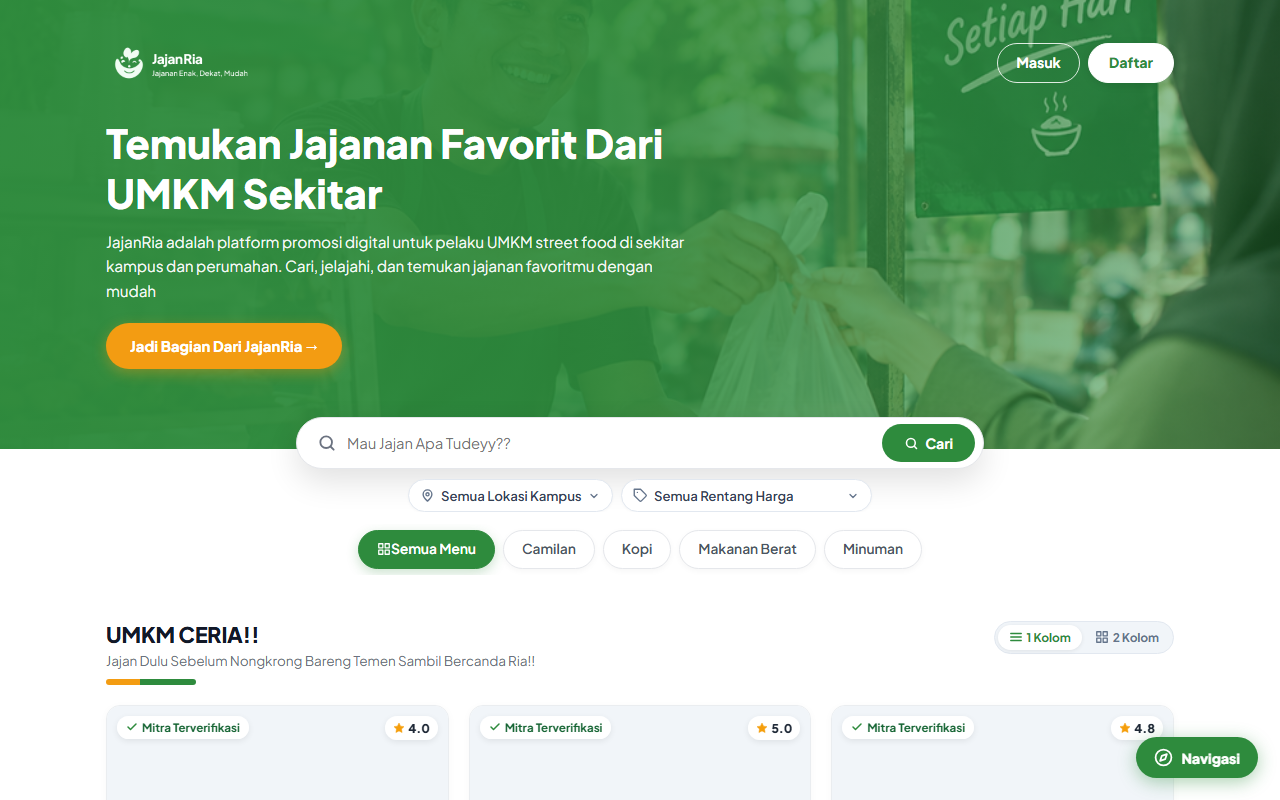
\includegraphics[width=0.92\textwidth]{assets/screens/01_landing.png}
\caption{Implementasi Halaman Beranda dan Katalog Utama}
\label{fig:ui-landing}
\end{figure}

\subsubsection{Halaman Masuk dan Pendaftaran Mitra Penjual}
Halaman masuk memfasilitasi autentikasi Pengunjung melalui \textit{Google Sign-In} (\textit{Firebase}) maupun tombol masuk dengan surel serta kata sandi untuk Penjual dan Admin. Sementara itu, halaman pendaftaran mitra menyediakan formulir tervalidasi dengan bidang nama pemilik, nama usaha, kontak, area, lokasi, unggah foto lapak, serta kata sandi. Kedua antarmuka tersebut ditunjukkan pada Gambar~\ref{fig:ui-auth}.

\begin{figure}[htbp]
\centering
\begin{minipage}[t]{0.48\textwidth}
  \centering
  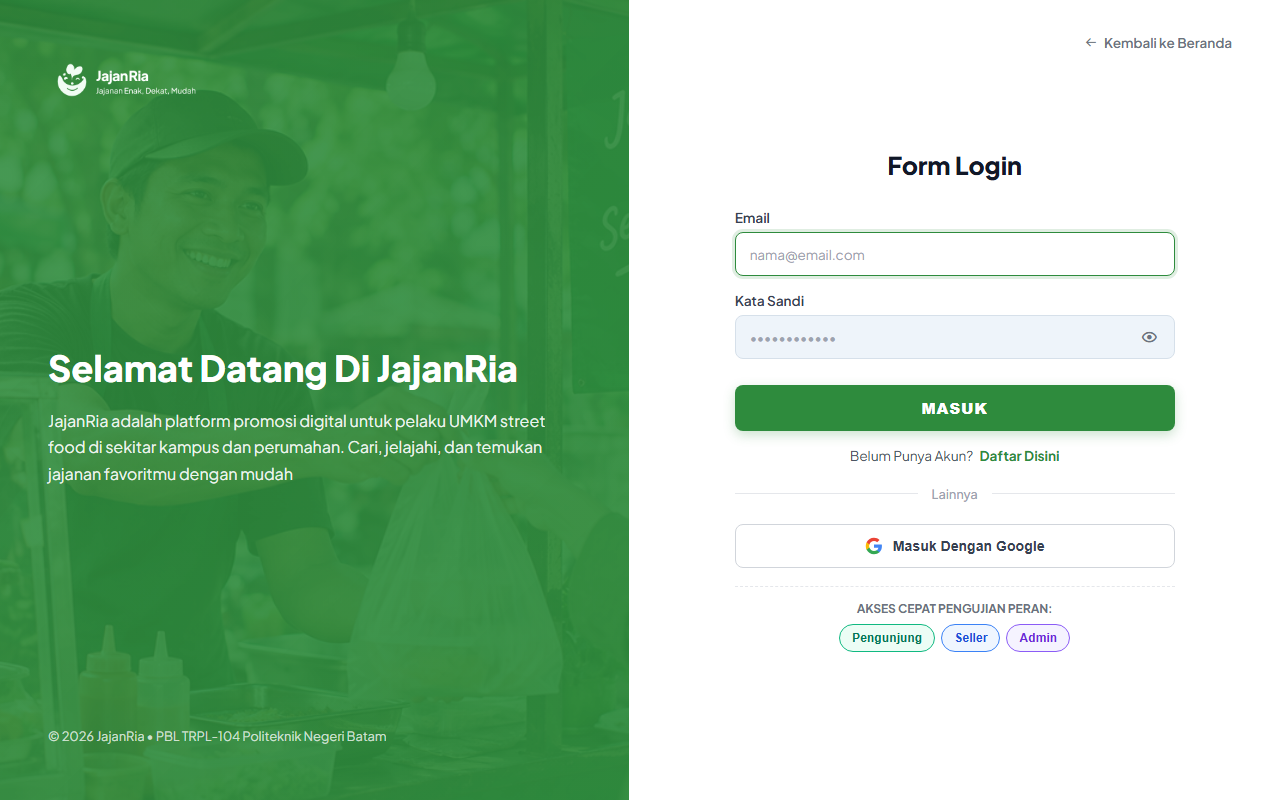
\includegraphics[width=\textwidth]{assets/screens/02_login.png}
  \par\small (a) Halaman Masuk
\end{minipage}\hfill
\begin{minipage}[t]{0.48\textwidth}
  \centering
  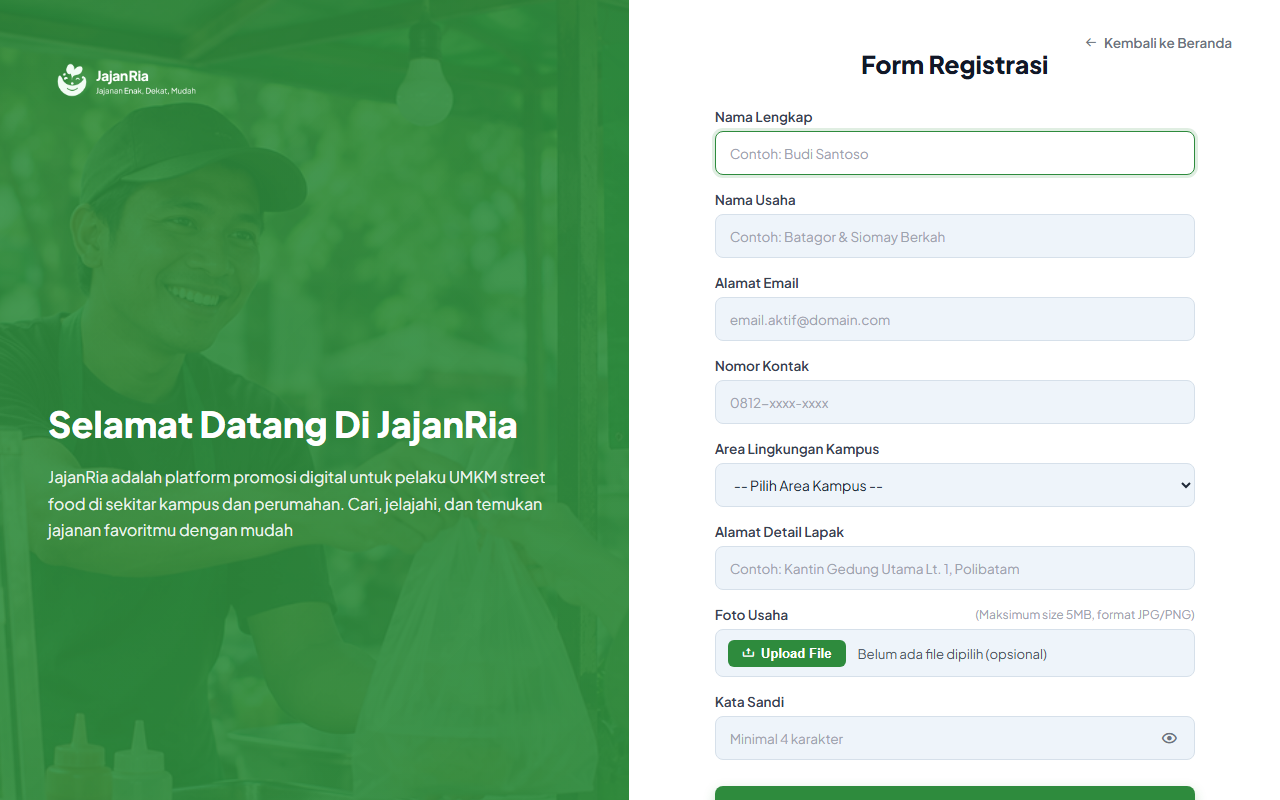
\includegraphics[width=\textwidth]{assets/screens/03_register.png}
  \par\small (b) Halaman Pendaftaran Mitra
\end{minipage}
\caption{Implementasi Antarmuka Autentikasi dan Registrasi Mitra UMKM}
\label{fig:ui-auth}
\end{figure}

\subsubsection{Halaman Detail Lapak, Keranjang, dan Modal Checkout}
Halaman detail lapak menyajikan informasi usaha, kelompok menu per kategori berikut penanda status habis, ulasan pembeli, serta bilah keranjang mengambang. Saat tombol ``Checkout \& Pembayaran'' dipilih, sistem membuka modal ringkasan pesanan, informasi pembayaran lapak, kolom unggah foto bukti bayar, serta catatan pesanan sebagaimana tampak pada Gambar~\ref{fig:ui-checkout}.

\begin{figure}[htbp]
\centering
\begin{minipage}[t]{0.48\textwidth}
  \centering
  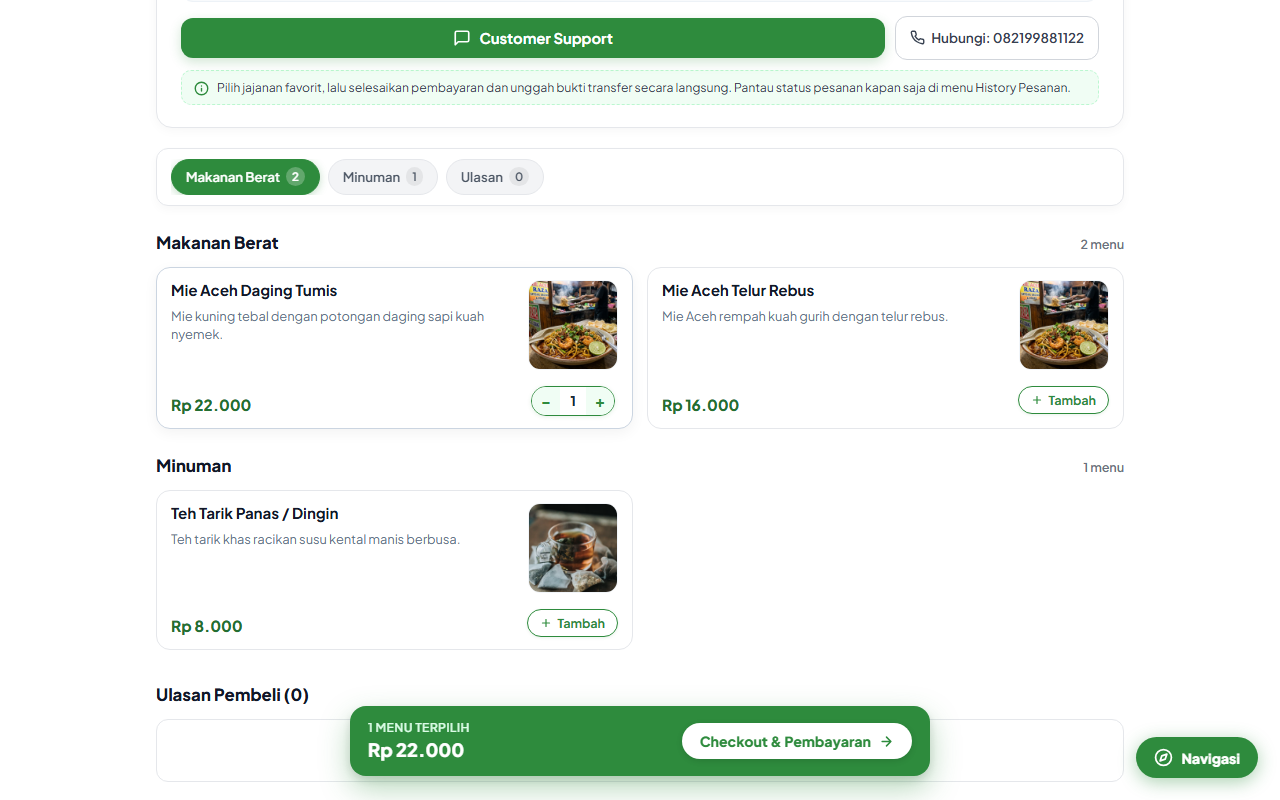
\includegraphics[width=\textwidth]{assets/screens/04_store_detail.png}
  \par\small (a) Detail Lapak \& Keranjang Belanja
\end{minipage}\hfill
\begin{minipage}[t]{0.48\textwidth}
  \centering
  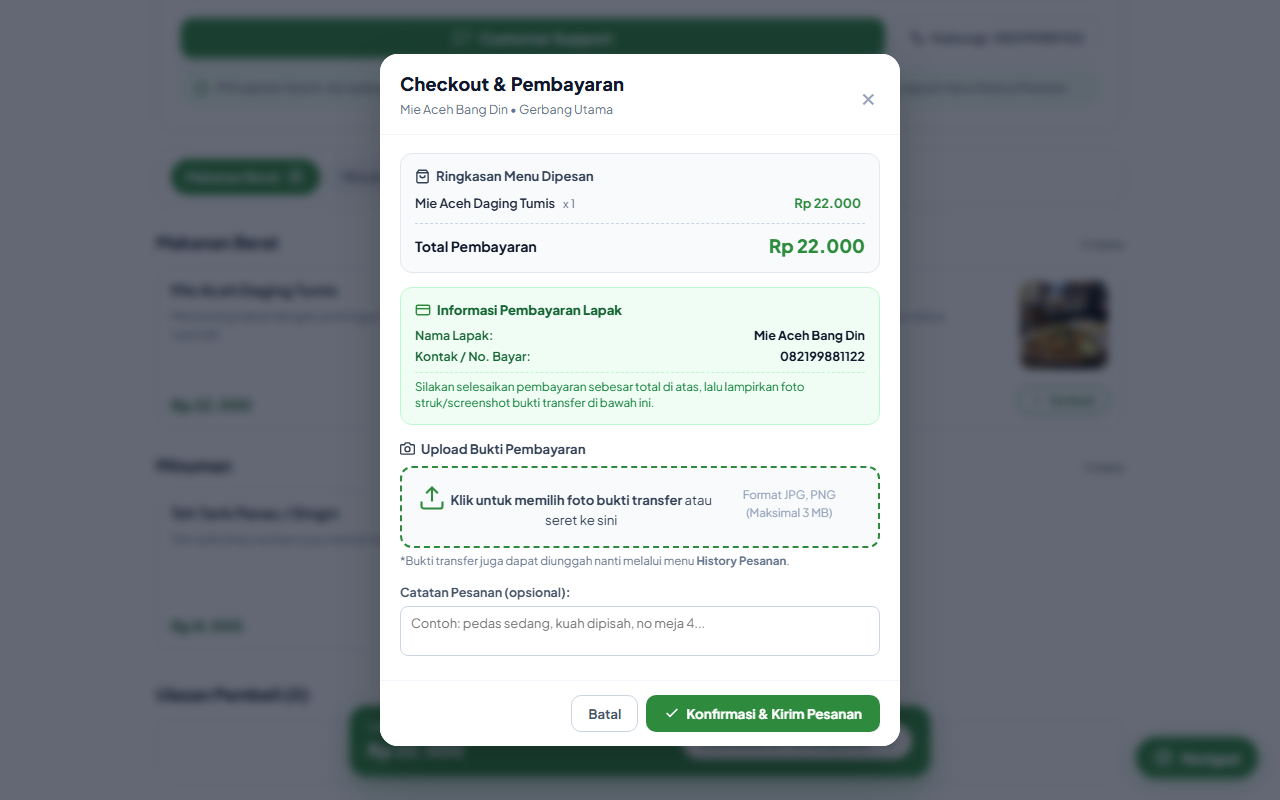
\includegraphics[width=\textwidth]{assets/screens/05_checkout_modal.png}
  \par\small (b) Modal \textit{Checkout} \& Pembayaran
\end{minipage}
\caption{Implementasi Detail Lapak UMKM dan Modal \textit{Checkout} Mandiri}
\label{fig:ui-checkout}
\end{figure}

\subsubsection{Laci History Pesanan dan Layanan Customer Support}
Pengunjung membuka menu peluncur \textit{Navigasi} di sudut kanan bawah untuk memantau transaksi pada laci \textit{History Pesanan}. Laci ini menampilkan status pesanan serta pembayaran, tombol unggah ulang bukti transfer, dan tombol ``Beri Penilaian'' saat pesanan berstatus \textit{selesai} dan \textit{lunas}. Saluran bantuan tersedia terpisah pada laci \textit{Customer Support} untuk berkirim pesan bersama Admin seperti pada Gambar~\ref{fig:ui-drawers}.

\begin{figure}[htbp]
\centering
\begin{minipage}[t]{0.48\textwidth}
  \centering
  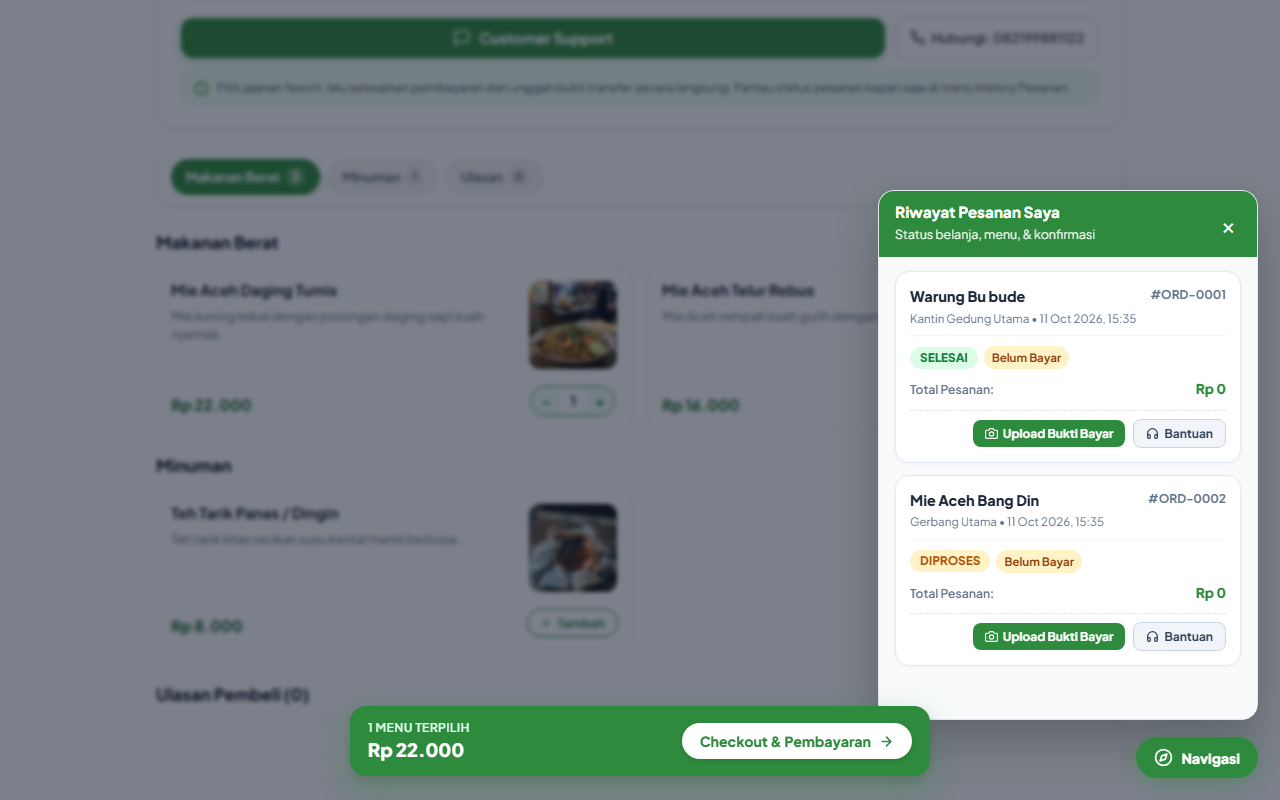
\includegraphics[width=\textwidth]{assets/screens/06_history_drawer.png}
  \par\small (a) Laci \textit{History Pesanan}
\end{minipage}\hfill
\begin{minipage}[t]{0.48\textwidth}
  \centering
  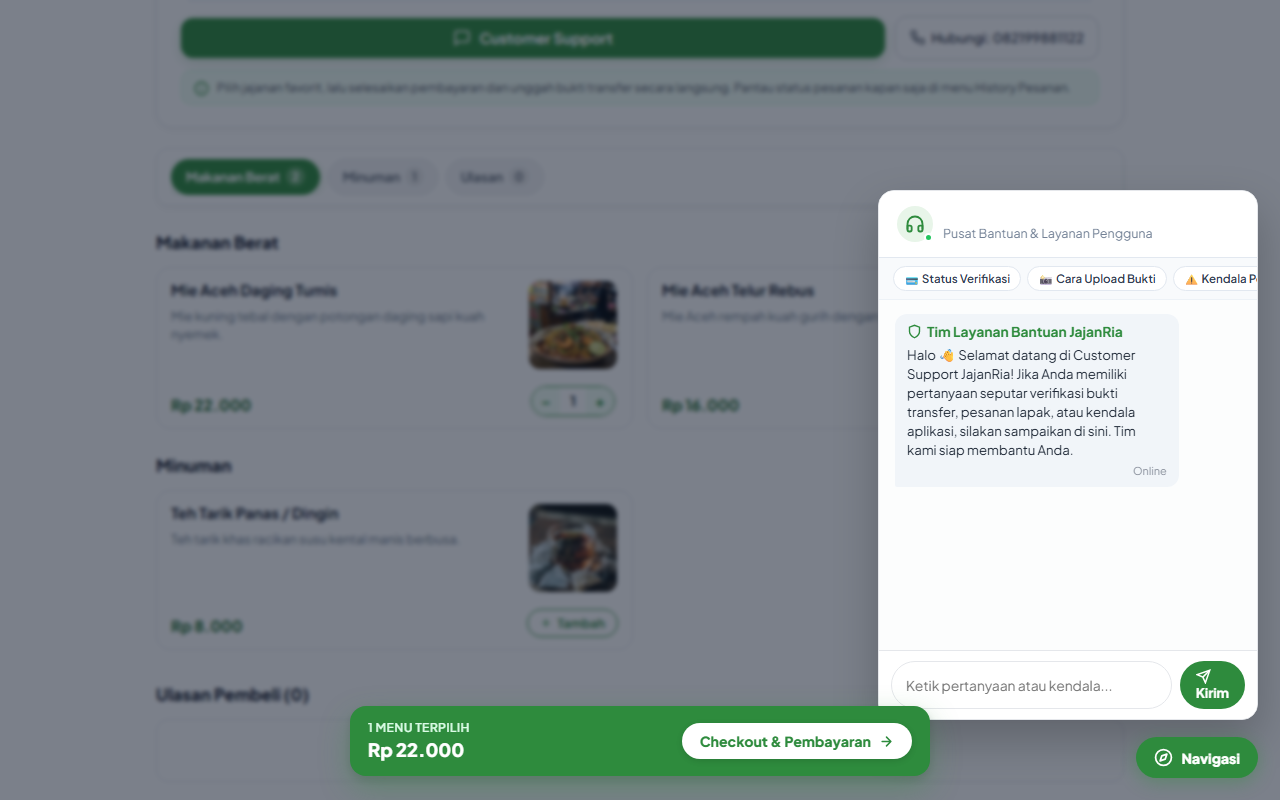
\includegraphics[width=\textwidth]{assets/screens/07_support_drawer.png}
  \par\small (b) Laci \textit{Customer Support}
\end{minipage}
\caption{Implementasi Laci \textit{History Pesanan} dan Pusat Bantuan Pelanggan}
\label{fig:ui-drawers}
\end{figure}

\subsubsection{Dasbor Penjual (Seller UMKM)}
Dasbor Penjual menyediakan lima tab fungsional yang menjaga posisi tab aktif setiap kali aksi dikirimkan, yaitu Ringkasan Toko, Kelola Menu \& Katalog, Pesan \& Pesanan, Profil Lapak UMKM, dan Rating \& Ulasan. Pada tab pesanan, rincian menu pesanan dan catatan pembeli tampil berdampingan, sedangkan tombol ``Selesai'' hanya aktif setelah Admin memverifikasi status pembayaran menjadi \textit{lunas}. Tampilan dasbor Penjual ditunjukkan pada Gambar~\ref{fig:ui-seller}.

\begin{figure}[htbp]
\centering
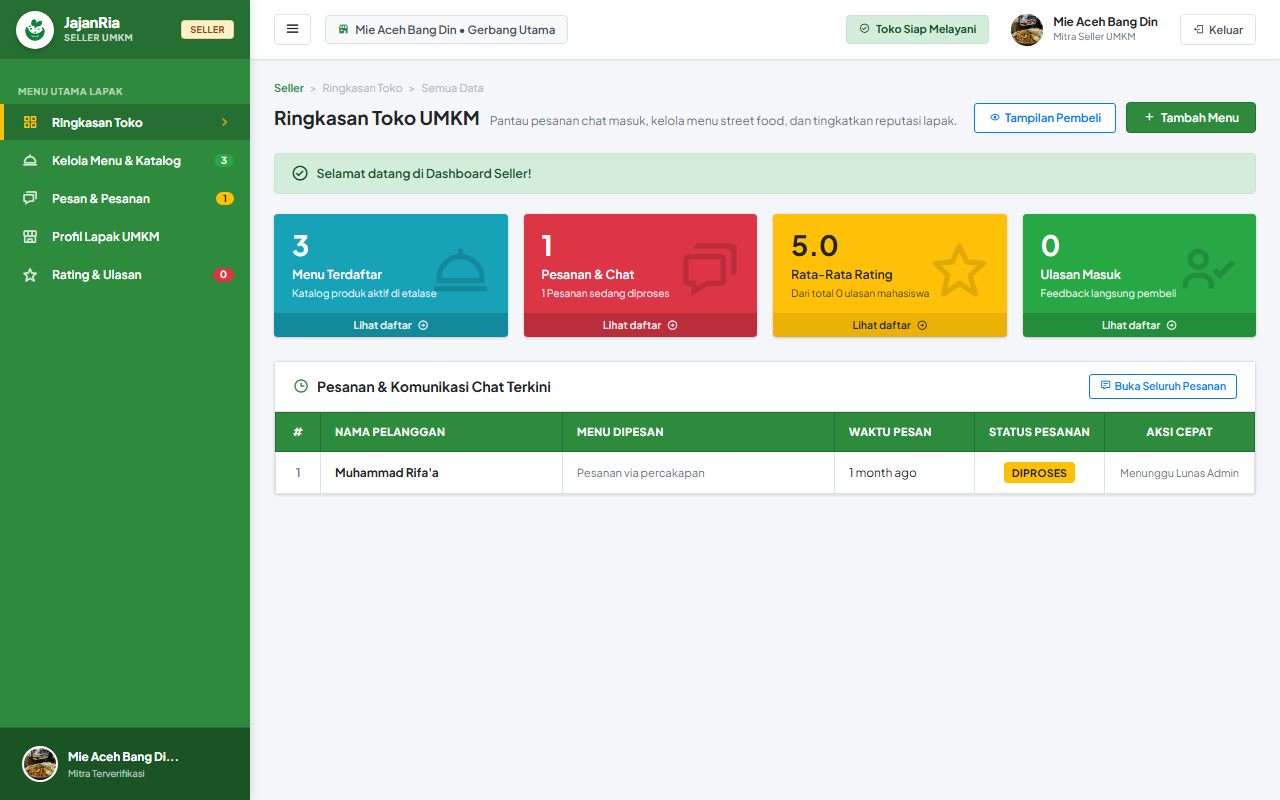
\includegraphics[width=0.90\textwidth]{assets/screens/08_seller_overview.png}
\par\vspace{0.2cm}\small (a) Tab Ringkasan Toko Penjual
\par\vspace{0.35cm}
\begin{minipage}[t]{0.48\textwidth}
  \centering
  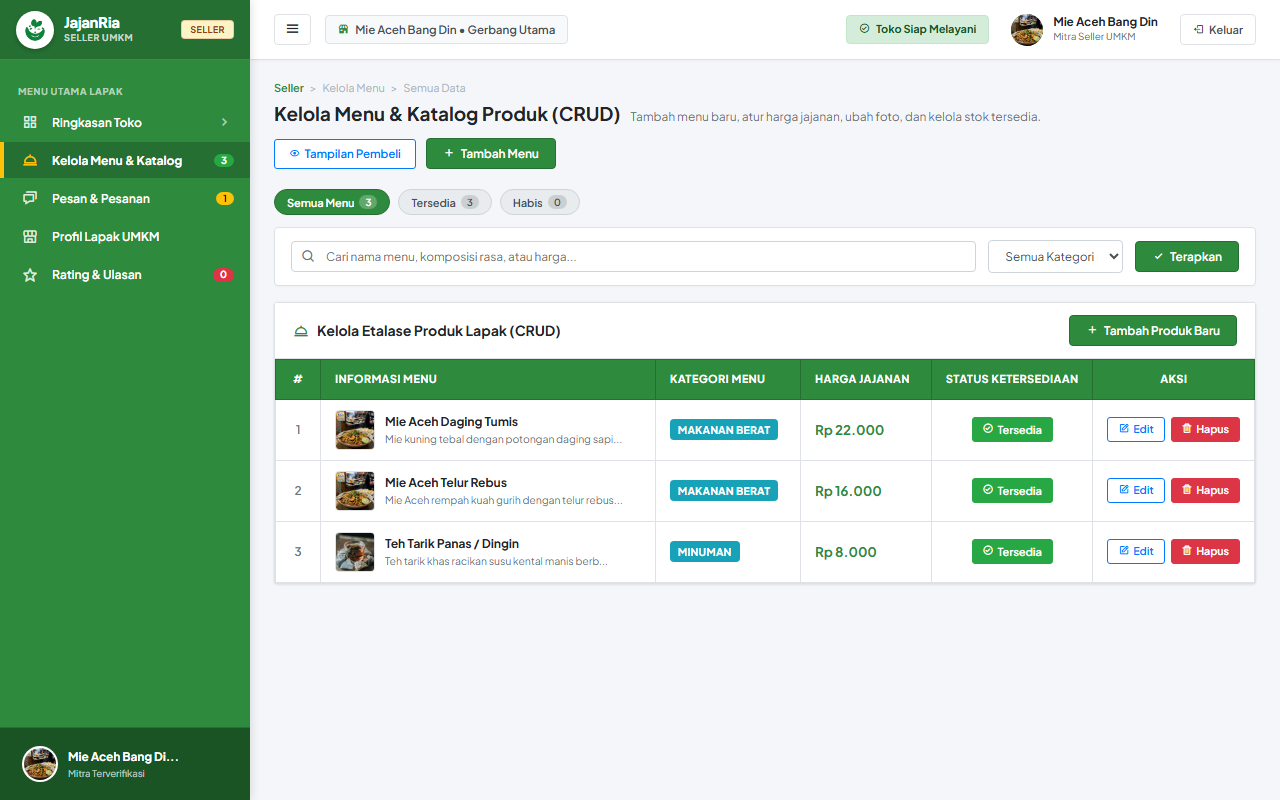
\includegraphics[width=\textwidth]{assets/screens/09_seller_products.png}
  \par\small (b) Tab Kelola Menu \& Ketersediaan
\end{minipage}\hfill
\begin{minipage}[t]{0.48\textwidth}
  \centering
  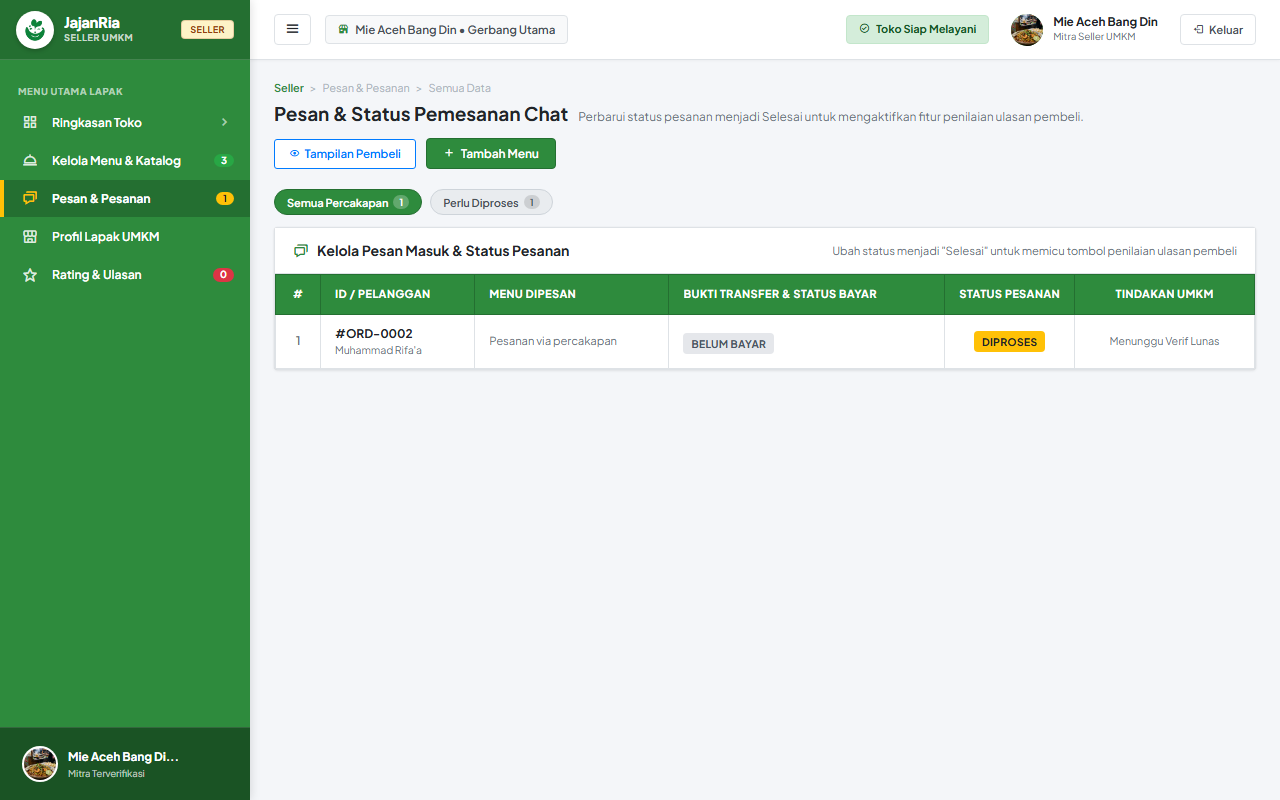
\includegraphics[width=\textwidth]{assets/screens/10_seller_orders.png}
  \par\small (c) Tab Daftar Pesanan \& Status Bayar
\end{minipage}
\caption{Implementasi Dasbor Operasional Penjual UMKM}
\label{fig:ui-seller}
\end{figure}

\subsubsection{Panel Administrator}
Panel Administrator menjadi pusat kendali platform dengan delapan tab terintegrasi: Monitoring \& Statistik, Verifikasi Seller Baru, Verifikasi Pembayaran, Kelola Mitra UMKM, Kelola Kategori Menu, Moderasi Ulasan, \textit{Customer Support}, dan Manajemen User. Seluruh tombol aksi kini bertahan pada tab aktif masing-masing, termasuk modal alasan penolakan bukti bayar dan proteksi hapus kategori berproduk aktif. Antarmuka panel Admin ditunjukkan pada Gambar~\ref{fig:ui-admin}.

\begin{figure}[htbp]
\centering
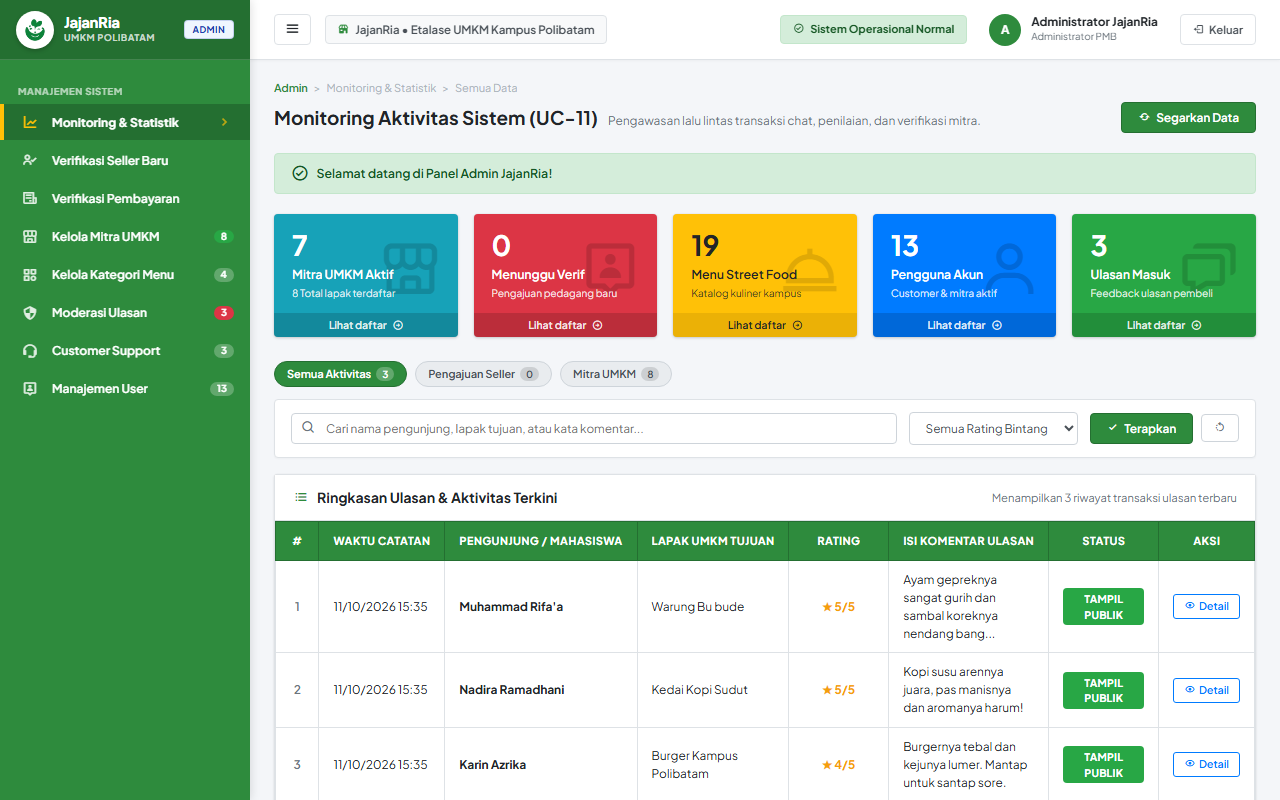
\includegraphics[width=0.90\textwidth]{assets/screens/11_admin_monitoring.png}
\par\vspace{0.2cm}\small (a) Tab Monitoring \& Statistik Platform
\par\vspace{0.35cm}
\begin{minipage}[t]{0.48\textwidth}
  \centering
  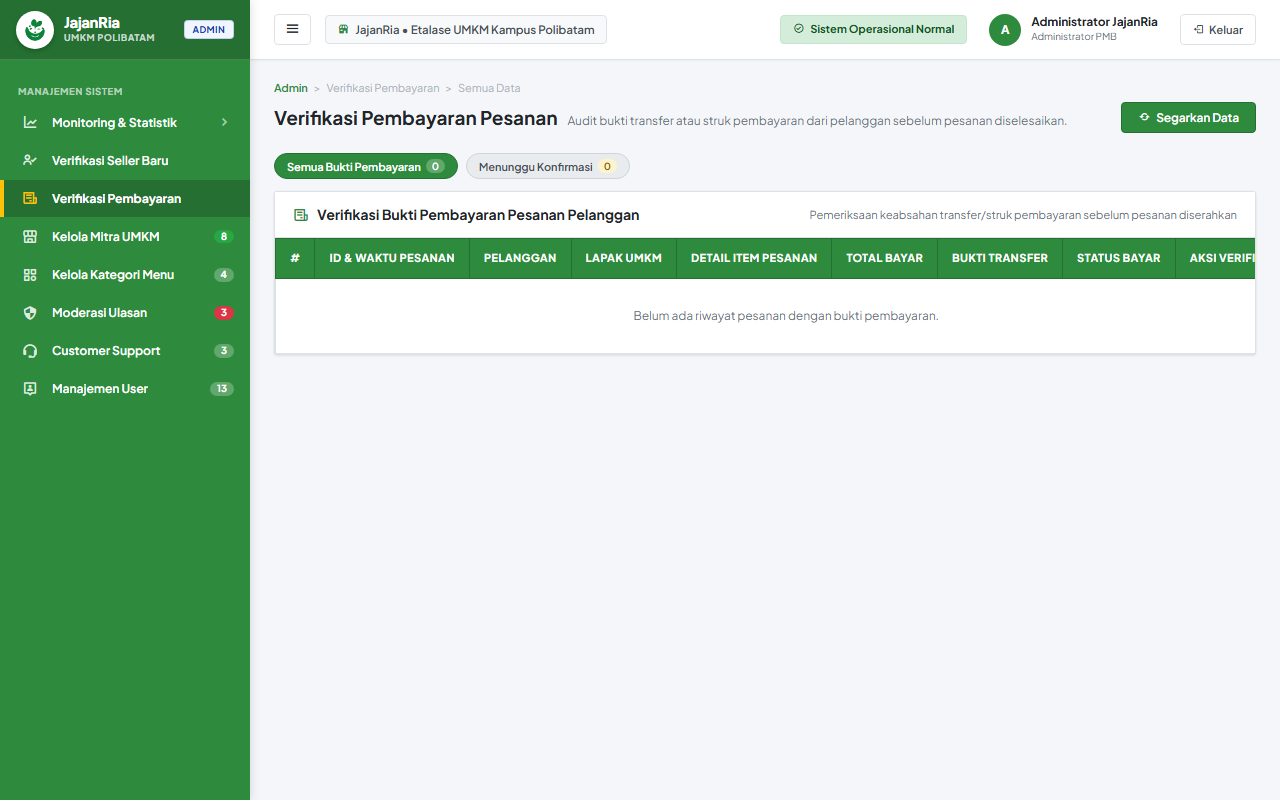
\includegraphics[width=\textwidth]{assets/screens/12_admin_payments.png}
  \par\small (b) Tab Verifikasi Pembayaran Manual
\end{minipage}\hfill
\begin{minipage}[t]{0.48\textwidth}
  \centering
  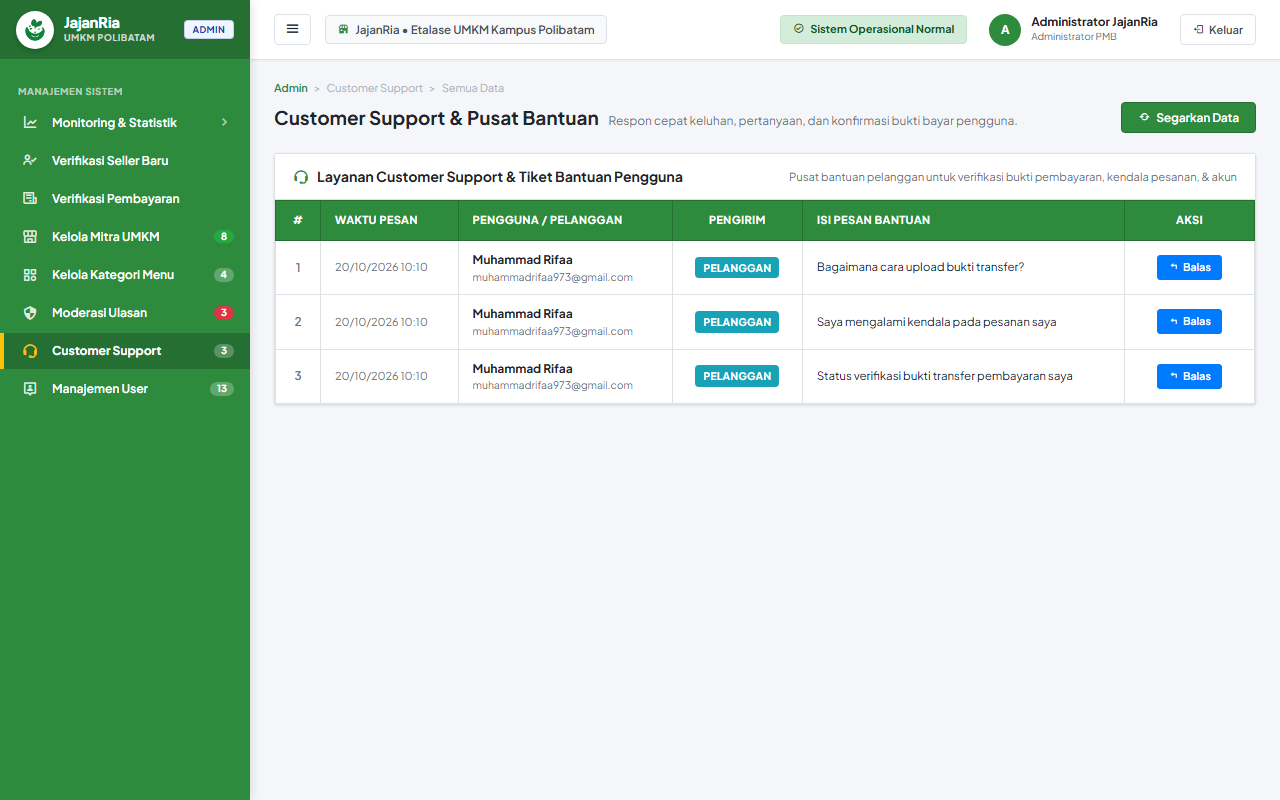
\includegraphics[width=\textwidth]{assets/screens/13_admin_support.png}
  \par\small (c) Tab Layanan \textit{Customer Support}
\end{minipage}
\caption{Implementasi Panel Administrator JajanRia}
\label{fig:ui-admin}
\end{figure}

\subsection{Implementasi Basis Data}

\subsubsection{Sistem Manajemen Basis Data dan Struktur Tabel}
Sistem JajanRia berjalan di atas sistem manajemen basis data relasional \textit{Structured Query Language} (SQL) MySQL versi \texttt{10.4.32-MariaDB} pada basis data \texttt{jajanria} dengan set karakter \texttt{utf8mb4\_unicode\_ci}. Skema basis data dibangun melalui 13 berkas migrasi Laravel~11 dan menghasilkan 16 tabel total. Tabel tersebut terdiri dari tujuh tabel domain aplikasi serta sembilan tabel kerangka kerja (\texttt{migrations}, \texttt{sessions}, \texttt{cache}, \texttt{cache\_locks}, \texttt{jobs}, \texttt{job\_batches}, \texttt{failed\_jobs}, \texttt{password\_\allowbreak reset\_tokens}, dan \texttt{users}). Inventaris tujuh tabel domain beserta volume baris aktual disajikan pada Tabel~\ref{tab:inventaris-db}.

\renewcommand{\arraystretch}{1.22}
\begin{longtable}{|L{2.8cm}|C{2.0cm}|L{\dimexpr\textwidth-2.8cm-2.0cm-6\tabcolsep-4\arrayrulewidth\relax}|}
\caption{Inventaris Tabel Domain Basis Data \texttt{jajanria}}
\label{tab:inventaris-db} \\
\hline
\rowcolor{TableHeadBg}
\textbf{Nama Tabel} & \textbf{Jumlah Baris} & \textbf{Fungsi Utama dalam Sistem} \\
\hline
\endfirsthead
\hline
\rowcolor{TableHeadBg}
\textbf{Nama Tabel} & \textbf{Jumlah Baris} & \textbf{Fungsi Utama dalam Sistem} \\
\hline
\endhead
\hline
\endfoot
\texttt{t\_user} & 13 & Akun Pengunjung, Penjual, dan Administrator berikut status verifikasi serta keaktifan. \\
\hline
\texttt{t\_umkm} & 8 & Profil lapak UMKM kuliner, lokasi rinci, kawasan area, kontak, dan foto lapak. \\
\hline
\texttt{t\_kategori} & 4 & Daftar kategori menu unik (\textit{Makanan Berat}, \textit{Camilan}, \textit{Minuman}, \textit{Kopi}). \\
\hline
\texttt{t\_produk} & 19 & Menu kuliner setiap UMKM beserta harga dan penanda ketersediaan (\texttt{tersedia}). \\
\hline
\texttt{t\_pesan} & 15 & Riwayat tiket \textit{Customer Support} (\texttt{id\_umkm = \textit{null}}) dan log pesan lama. \\
\hline
\texttt{t\_pesanan} & 7 & Transaksi pesanan langsung berisi \texttt{items\_detail}, catatan, bukti bayar, dan status. \\
\hline
\texttt{t\_ulasan} & 3 & Peringkat (1--5), komentar pembeli, balasan penjual, serta status moderasi. \\
\hline
\end{longtable}

\subsubsection{Contoh Data Aktual Basis Data}
Cuplikan isi nyata dari basis data \texttt{jajanria} untuk tabel pengguna, UMKM, kategori, produk, dan ulasan ditampilkan pada Tabel~\ref{tab:contoh-data-db}. Kolom kredensial seperti \textit{hash} kata sandi maupun pengenal internal Firebase tidak dicantumkan demi menjaga keamanan data.

\renewcommand{\arraystretch}{1.20}
\begin{longtable}{|L{2.2cm}|L{1.55cm}|L{\dimexpr\textwidth-2.2cm-1.55cm-6\tabcolsep-4\arrayrulewidth\relax}|}
\caption{Cuplikan Data Aktual pada Basis Data \texttt{jajanria}}
\label{tab:contoh-data-db} \\
\hline
\rowcolor{TableHeadBg}
\textbf{Tabel} & \textbf{ID Baris} & \textbf{Cuplikan Nilai Kolom Utama} \\
\hline
\endfirsthead
\hline
\rowcolor{TableHeadBg}
\textbf{Tabel} & \textbf{ID Baris} & \textbf{Cuplikan Nilai Kolom Utama} \\
\hline
\endhead
\hline
\endfoot
\texttt{t\_user} & \texttt{id=1} & \texttt{nama="Administrator JajanRia"}, \texttt{role="admin"}, \texttt{status\_verifikasi="terverifikasi"}, \texttt{is\_active=1} \\
\hline
\texttt{t\_user} & \texttt{id=6} & \texttt{nama="Pemilik Mie Aceh Bang Din"}, \texttt{role="seller"}, \texttt{status\_verifikasi="terverifikasi"}, \texttt{is\_active=1} \\
\hline
\texttt{t\_umkm} & \texttt{id=2} & \texttt{nama\_usaha="Mie Aceh Bang Din"}, \texttt{area="Gerbang Utama"}, \texttt{kontak="082199881122"} \\
\hline
\texttt{t\_umkm} & \texttt{id=4} & \texttt{nama\_usaha="Kedai Kopi Sudut"}, \texttt{area="Ruko KDA"}, \texttt{kontak="087733119002"} \\
\hline
\texttt{t\_kategori} & \texttt{id=1..4} & \texttt{Makanan Berat} (1), \texttt{Camilan} (2), \texttt{Minuman} (3), \texttt{Kopi} (4) \\
\hline
\texttt{t\_produk} & \texttt{id=5} & \texttt{id\_umkm=2}, \texttt{id\_kategori=1}, \texttt{nama\_produk="Mie Aceh Daging Tumis"}, \texttt{harga=22000.00}, \texttt{tersedia=1} \\
\hline
\texttt{t\_produk} & \texttt{id=7} & \texttt{id\_umkm=2}, \texttt{id\_kategori=3}, \texttt{nama\_produk="Teh Tarik Panas / Dingin"}, \texttt{harga=8000.00}, \texttt{tersedia=1} \\
\hline
\texttt{t\_ulasan} & \texttt{id=1} & \texttt{id\_pesanan=1}, \texttt{id\_umkm=1}, \texttt{rating=5}, \texttt{disembunyikan=0} \\
\hline
\end{longtable}

\subsubsection{Contoh Kueri yang Diimplementasikan}
Operasi akses data memakai pemetaan relasional objek (\textit{Object-Relational Mapping} atau ORM) Eloquent pada lapisan kontroler sehingga terlindung oleh pengikatan parameter untuk mencegah injeksi kueri SQL. Tiga kueri inti pada alur pencarian, transaksi \textit{checkout}, dan verifikasi pembayaran disajikan pada Kode~\ref{lst:kueri-app}.

\begin{lstlisting}[language=PHP, caption={Contoh Kueri Aplikasi pada Kontroler JajanRia}, label={lst:kueri-app}]
// 1. Kueri Katalog Publik Terverifikasi & Rating (UmkmController::index)
$lapak = Umkm::tampil()
    ->with(['produk.kategori'])
    ->withAvg(['ulasan as rata_rating' => $ulasanTampil], 'rating')
    ->withCount(['ulasan as jumlah_ulasan' => $ulasanTampil])
    ->when(!$mencari, fn ($query) => $query->whereIn('area', $sekitar))
    ->orderBy('nama_usaha')->get();

// 2. Validasi Menu & Hitung Harga Server saat Checkout (ChatController::checkoutOrder)
$produk = Produk::where('id_produk', $prodId)
    ->where('id_umkm', $idUmkm)->first();
$harga = (int) round($produk->harga);

// 3. Verifikasi Pembayaran Terpusat oleh Admin (AdminController::verifyPayment)
$pesanan = Pesanan::findOrFail($idPesanan);
$pesanan->update([
    'status_pembayaran' => $status,
    'catatan_admin'     => $catatan ?: null,
]);
\end{lstlisting}

\clearpage
\section{Perencanaan, Deskripsi dan Hasil Uji Perangkat Lunak}

\subsection{Rencana Pengujian}

Pengujian fungsional dilakukan dengan pendekatan \textit{black-box} terhadap seluruh skenario \textit{use case} yang diimplementasikan (\texttt{UC-01} s.d.\ \texttt{UC-13}). Pengujian turut mencakup verifikasi persistensi tab pasca-aksi pada dasbor Penjual serta Admin, audit protokol transfer hiperteks (\textit{Hypertext Transfer Protocol}) untuk metode permintaan \texttt{GET} dan \texttt{POST}, serta pengujian unit/fitur bawaan Laravel. Eksekusi pengujian otomatis dijalankan pada tanggal 19 November 2026 memakai \textit{Playwright} pada peramban \textit{Chromium} terhadap klon basis data terisolasi (\texttt{jajanria\_test}) agar data usaha mikro, kecil, dan menengah (UMKM) pada basis data utama tetap aman. Daftar kasus uji dirangkum pada Tabel~\ref{tab:rencana-pengujian}.

\renewcommand{\arraystretch}{1.22}
\begin{longtable}{|C{1.55cm}|L{\dimexpr\textwidth-1.55cm-2.0cm-1.7cm-2.1cm-2.3cm-12\tabcolsep-7\arrayrulewidth\relax}|C{2.0cm}|C{1.7cm}|C{2.1cm}|L{2.3cm}|}
\caption{Rencana Pengujian Fungsional Sistem JajanRia}
\label{tab:rencana-pengujian} \\
\hline
\rowcolor{TableHeadBg}
\textbf{Nomor Uji} & \textbf{Nama Kasus Uji} & \textbf{Kebutuhan} & \textbf{Jenis Uji} & \textbf{Tanggal Uji} & \textbf{Nama Penguji} \\
\hline
\endfirsthead
\hline
\rowcolor{TableHeadBg}
\textbf{Nomor Uji} & \textbf{Nama Kasus Uji} & \textbf{Kebutuhan} & \textbf{Jenis Uji} & \textbf{Tanggal Uji} & \textbf{Nama Penguji} \\
\hline
\endhead
\hline
\endfoot
KU-001 & Autentikasi Admin dan Penjual valid serta penolakan akun nonaktif atau sandi salah & F001 & \textit{Black-box} & 19/11/2026 & Tim Penguji TRPL-104 \\
\hline
KU-002 & Registrasi mandiri mitra Penjual baru melalui formulir pendaftaran mitra & F001 & \textit{Black-box} & 19/11/2026 & Tim Penguji TRPL-104 \\
\hline
KU-003 & Pencarian kata kunci, penyaring katalog, dan halaman detail lapak UMKM & F002--F005 & \textit{Black-box} & 19/11/2026 & Tim Penguji TRPL-104 \\
\hline
KU-004 & \textit{Checkout} keranjang, kalkulasi harga di server, dan penolakan menu habis & F006 & \textit{Black-box} & 19/11/2026 & Tim Penguji TRPL-104 \\
\hline
KU-005 & Unggah foto bukti pembayaran transfer saat \textit{checkout} dan via \textit{History Pesanan} & F007 & \textit{Black-box} & 19/11/2026 & Tim Penguji TRPL-104 \\
\hline
KU-006 & Verifikasi bukti pembayaran terpusat oleh Admin (Setujui \textit{Lunas} \& Tolak via modal alasan) & F008 & \textit{Black-box} & 19/11/2026 & Tim Penguji TRPL-104 \\
\hline
KU-007 & Penjual menyelesaikan pesanan \textit{Self Pick-up} dan larangan sebelum status \textit{lunas} & F009 & \textit{Black-box} & 19/11/2026 & Tim Penguji TRPL-104 \\
\hline
KU-008 & Pemicu tombol ``Beri Penilaian'' (\textit{selesai} dan \textit{lunas}), pengiriman ulasan, serta balasan Penjual & F010--F012 & \textit{Black-box} & 19/11/2026 & Tim Penguji TRPL-104 \\
\hline
KU-009 & Pengelolaan menu, profil lapak UMKM, dan status ketersediaan menu Penjual & F013--F014 & \textit{Black-box} & 19/11/2026 & Tim Penguji TRPL-104 \\
\hline
KU-010 & Verifikasi calon Penjual, proteksi hapus kategori berproduk aktif, dan moderasi ulasan Admin & F015--F017, F019 & \textit{Black-box} & 19/11/2026 & Tim Penguji TRPL-104 \\
\hline
KU-011 & Komunikasi layanan \textit{Customer Support} dua arah antara Pengunjung dan Admin Support & F018 & \textit{Black-box} & 19/11/2026 & Tim Penguji TRPL-104 \\
\hline
KU-012 & Otorisasi akses Panel Administrator, Dasbor Penjual, dan isolasi kepemilikan ulasan & F020 & \textit{Black-box} & 19/11/2026 & Tim Penguji TRPL-104 \\
\hline
\end{longtable}

\subsection{Deskripsi dan Hasil Uji}

% Macro kotak hasil uji standar Halaman 41 Format laporan Polibatam
\newcommand{\printtestcase}[9]{%
\needspace{9cm}
\noindent
\renewcommand{\arraystretch}{1.20}
\begin{tabularx}{\textwidth}{|L{3.2cm}|Y|Y|}
\hline
\rowcolor{TableHeadBg}
\textbf{Identifikasi} & \multicolumn{2}{l|}{\textbf{#1}} \\
\hline
\textbf{Nama Kasus Uji} & \multicolumn{2}{>{\raggedright\arraybackslash}p{\dimexpr\textwidth-3.2cm-4\tabcolsep-3\arrayrulewidth\relax}|}{#2} \\
\hline
\textbf{Deskripsi} & \multicolumn{2}{>{\raggedright\arraybackslash}p{\dimexpr\textwidth-3.2cm-4\tabcolsep-3\arrayrulewidth\relax}|}{#3} \\
\hline
\textbf{Kondisi Awal} & \multicolumn{2}{>{\raggedright\arraybackslash}p{\dimexpr\textwidth-3.2cm-4\tabcolsep-3\arrayrulewidth\relax}|}{#4} \\
\hline
\textbf{Tanggal Pengujian} & \multicolumn{2}{l|}{#5} \\
\hline
\textbf{Penguji} & \multicolumn{2}{l|}{#6} \\
\hline
\rowcolor{RowShade}
\multicolumn{3}{|c|}{\textbf{Skenario Pengujian}} \\
\hline
\multicolumn{3}{|>{\raggedright\arraybackslash}p{\dimexpr\textwidth-2\tabcolsep-2\arrayrulewidth\relax}|}{#7} \\
\hline
\rowcolor{TableHeadBg}
\textbf{Hasil yang Diharapkan} & \textbf{Hasil Pengamatan} & \textbf{Kesimpulan} \\
\hline
#8 & #9 & \textbf{\color{JajanGreen}Sesuai (PASS)} \\
\hline
\end{tabularx}
\vspace{0.35cm}
}

Rincian skenario, hasil yang diharapkan, hasil pengamatan aktual, dan kesimpulan untuk seluruh 12 kasus uji fungsional disajikan pada tabel identifikasi di bawah ini.

\printtestcase{KU-001}{Autentikasi Admin dan Penjual Valid serta Penolakan Sandi Salah / Akun Nonaktif}
{Menguji proses masuk memakai surel dan kata sandi valid maupun penolakan kata sandi literal yang bukan milik akun, serta pemilih akun cepat aktif.}
{Akun Admin, Penjual aktif, dan Pengunjung tersedia di basis data uji.}
{19 November 2026}{Tim Penguji TRPL-104 (Playwright \& Audit HTTP)}
{\begin{uclist}
  \item Kirim permintaan masuk memakai surel aktif dengan kata sandi tidak valid (\texttt{wrongpass} dan literal \texttt{'password'}).
  \item Klik tombol akses cepat peran Penjual pada halaman masuk.
  \item Masuk menggunakan kredensial Administrator valid.
\end{uclist}}
{Percobaan sandi salah ditolak ke halaman masuk; tombol cepat Penjual memilih lapak aktif; Admin masuk ke Panel Administrator.}
{Percobaan sandi literal \texttt{'password'} dialihkan kembali ke halaman masuk (\texttt{HTTP 302}); akses cepat Penjual masuk ke lapak aktif Mie Aceh Bang Din; Admin masuk ke Panel Administrator.}

\printtestcase{KU-002}{Registrasi Mandiri Mitra Penjual Baru melalui Formulir Pendaftaran}
{Menguji pengiriman formulir pendaftaran mitra UMKM dengan seluruh bidang selaras beserta validasinya.}
{Pengguna belum masuk akun dan membuka halaman pendaftaran mitra.}
{19 November 2026}{Tim Penguji TRPL-104 (Playwright E2E)}
{\begin{uclist}
  \item Isi nama pemilik, nama usaha (\texttt{Bakso Budi Kampus}), surel baru, nomor kontak, area (\texttt{Tower A}), alamat lokasi, dan kata sandi.
  \item Tekan tombol daftar mitra (\texttt{DAFTAR MITRA}).
  \item Periksa halaman tujuan dan status verifikasi pengguna pada Panel Administrator.
\end{uclist}}
{Pengguna dialihkan ke halaman masuk dengan spanduk sukses, serta calon mitra tercatat pada antrean verifikasi Admin.}
{Pengalihan ke halaman masuk berhasil dengan spanduk ``Pendaftaran Mitra UMKM berhasil!'', dan data \texttt{Bakso Budi Kampus} muncul di tab verifikasi Admin.}

\printtestcase{KU-003}{Pencarian Kata Kunci, Penyaring Katalog, dan Halaman Detail Lapak}
{Menguji tampilan katalog beranda, penyaringan, serta pemunculan lapak terverifikasi baru di halaman publik.}
{Mitra baru (\texttt{Bakso Budi Kampus}) telah disetujui Admin pada basis data uji.}
{19 November 2026}{Tim Penguji TRPL-104 (Playwright E2E)}
{\begin{uclist}
  \item Buka halaman beranda katalog sebagai Pengunjung dan cari lapak terverifikasi baru.
  \item Buka halaman detail lapak dan periksa kelompok menu serta status ketersediaan produk.
\end{uclist}}
{Lapak terverifikasi baru tampil di katalog publik beranda dan rincian menu tampil pada halaman detail lapak.}
{Lapak \texttt{Bakso Budi Kampus} tampil di katalog utama; halaman detail lapak memuat daftar menu per kategori dan penanda menu habis.}

\printtestcase{KU-004}{Checkout Keranjang, Kalkulasi Harga Server, dan Blokir Menu Habis}
{Menguji konsistensi nominal pada modal \textit{checkout}, validasi harga asli server, penyimpanan catatan pembeli, dan penolakan menu berstatus habis.}
{Pengunjung masuk akun dan membuka halaman detail lapak dengan salah satu menu tersedia dan satu menu berstatus habis.}
{19 November 2026}{Tim Penguji TRPL-104 (Playwright \& Audit HTTP)}
{\begin{uclist}
  \item Tambahkan 1 porsi menu (Rp22.000) ke keranjang lalu buka modal \textit{checkout} dan periksa total tagihan pada ringkasan modal.
  \item Kirim permintaan \textit{checkout} dengan nominal harga manipulatif (Rp1) untuk 2 porsi menu Rp22.000.
  \item Kirim permintaan \textit{checkout} untuk menu berstatus habis.
\end{uclist}}
{Modal menampilkan \texttt{Rp 22.000}; server mengabaikan harga manipulatif dan menghitung total Rp44.000; menu habis ditolak (\texttt{HTTP 422}).}
{Terbaca \texttt{'Rp 22.000'} di modal; permintaan \textit{checkout} mengembalikan \texttt{HTTP 200} dengan total tercatat \texttt{44000}; menu habis ditolak \texttt{HTTP 422}.}

\printtestcase{KU-005}{Unggah Foto Bukti Pembayaran Saat Checkout dan melalui History Pesanan}
{Menguji dua skenario pembayaran: melampirkan bukti langsung saat \textit{checkout}, serta \textit{checkout} tanpa bukti lalu mengunggah dari \textit{History Pesanan}.}
{Pengunjung telah masuk akun pada sesi aktif.}
{19 November 2026}{Tim Penguji TRPL-104 (Playwright E2E)}
{\begin{uclist}
  \item Lakukan \textit{checkout} pada lapak pertama disertai berkas gambar bukti bayar (\texttt{WF-01}).
  \item Lakukan \textit{checkout} tanpa foto pada lapak kedua, lalu buka laci \textit{History Pesanan} dan unggah foto bukti transfer (\texttt{WF-02}).
\end{uclist}}
{Pesanan langsung berstatus pembayaran \textit{Menunggu Verifikasi} dan status pesanan \textit{Diproses}; unggah susulan dari History berhasil.}
{Pesanan tercatat di \textit{History Pesanan} dengan status \textit{Menunggu Verifikasi} dan \textit{Diproses}, serta unggah susulan berhasil.}

\printtestcase{KU-006}{Verifikasi Bukti Pembayaran Terpusat oleh Admin (Setujui dan Tolak via Modal)}
{Menguji pengubahan status pembayaran oleh Admin dari tab pembayaran, termasuk pembukaan modal alasan penolakan serta persistensi tab.}
{Terdapat pesanan berstatus menunggu verifikasi pada basis data uji.}
{19 November 2026}{Tim Penguji TRPL-104 (Playwright E2E)}
{\begin{uclist}
  \item Masuk sebagai Admin lalu buka tab Verifikasi Pembayaran pada Panel Administrator.
  \item Tekan tombol Tolak untuk membuka modal penolakan pembayaran, isi alasan penolakan, lalu simpan.
  \item Tekan tombol Setujui (\textit{Lunas}) pada pesanan uji berikutnya.
\end{uclist}}
{Modal penolakan terbuka normal, status pembayaran diperbarui menjadi \textit{ditolak}/\textit{lunas}, dan tampilan tetap bertahan pada tab Verifikasi Pembayaran.}
{Modal tolak terbuka mulus, kedua aksi berhasil mengubah status pembayaran dan posisi halaman tetap berada di tab Verifikasi Pembayaran.}

\printtestcase{KU-007}{Penjual Menyelesaikan Pesanan Self Pick-up setelah Pembayaran Lunas}
{Menguji penampilan rincian item dan catatan pembeli di tabel Penjual, penguncian tombol Selesai sebelum lunas, dan penyelesaian setelah lunas.}
{Terdapat pesanan belum lunas dan pesanan lunas milik lapak Mie Aceh Bang Din.}
{19 November 2026}{Tim Penguji TRPL-104 (Playwright \& Audit HTTP)}
{\begin{uclist}
  \item Buka tab Pesan \& Pesanan pada Dasbor Penjual dan periksa kolom rincian menu, catatan pembeli, serta tombol status.
  \item Lakukan upaya mengubah status pesanan menjadi \textit{selesai} pada pesanan yang belum \textit{lunas}.
  \item Klik tombol Selesai pada pesanan yang telah diverifikasi \textit{lunas} oleh Admin.
\end{uclist}}
{Nama menu dan catatan tampil; pesanan belum lunas terkunci dan ditolak server; pesanan lunas berubah \textit{selesai} dan tetap berada di tab Pesan \& Pesanan.}
{Nama menu serta catatan pembeli tampil; penolakan sebelum lunas tampil; pesanan lunas berubah menjadi \textit{selesai} dan tampilan tetap di tab Pesan \& Pesanan.}

\printtestcase{KU-008}{Pemicu Tombol ``Beri Penilaian'' (Selesai + Lunas), Kirim Ulasan, dan Balasan Penjual}
{Menguji pemicu penilaian dan penolakan ulasan belum lunas. Diuji pula penyimpanan ulasan di History serta blokir balasan ulasan tersembunyi (\texttt{UC-08}).}
{Terdapat pesanan belum lunas, pesanan \textit{selesai} dan \textit{lunas}, serta satu ulasan disembunyikan Admin.}
{19 November 2026}{Tim Penguji TRPL-104 (Playwright \& Audit HTTP)}
{\begin{uclist}
  \item Kirim permintaan pengiriman ulasan untuk pesanan yang pembayarannya belum \textit{lunas}.
  \item Buka \textit{History Pesanan} untuk pesanan \textit{selesai} dan \textit{lunas}, klik ``Beri Penilaian'', lalu kirim bintang 5 dan komentar.
  \item Masuk sebagai Penjual pada tab Rating \& Ulasan, balas ulasan tampil, lalu coba balas ulasan yang disembunyikan Admin (\texttt{UC-08}).
\end{uclist}}
{Permintaan menolak ulasan belum lunas (\texttt{HTTP 400}); tombol penilaian muncul saat \textit{selesai} serta \textit{lunas}; balasan ulasan tersembunyi ditolak.}
{Ulasan belum lunas ditolak \texttt{HTTP 400}; tombol ``Beri Penilaian'' muncul dan tetap di laci History; balasan pada ulasan disembunyikan ditolak pesan galat.}

\printtestcase{KU-009}{Pengelolaan Menu, Profil Lapak UMKM, dan Ketersediaan Menu Penjual}
{Menguji tambah/ubah/hapus/toggle produk dan pembaruan profil termasuk area luar sekitar kampus, serta persistensi tab Penjual.}
{Penjual aktif masuk ke Dasbor Penjual.}
{19 November 2026}{Tim Penguji TRPL-104 (Playwright E2E)}
{\begin{uclist}
  \item Pada tab Kelola Menu \& Katalog, tambah menu baru, klik ubah ketersediaan (\textit{Tersedia}/\textit{Habis}), sunting menu, lalu hapus menu.
  \item Pada tab Profil Lapak UMKM, perbarui profil lapak lalu tekan simpan.
\end{uclist}}
{Seluruh operasi dan simpan profil berhasil tersimpan di basis data serta mempertahankan posisi tab aksi masing-masing.}
{Seluruh 9 skenario persistensi tab Penjual (termasuk 4 aksi produk, profil, pesanan, dan ulasan + muat ulang F5) berstatus \textbf{PASS}.}

\printtestcase{KU-010}{Verifikasi Calon Penjual, Proteksi Hapus Kategori (\texttt{UC-10}), dan Moderasi Ulasan Admin}
{Menguji persetujuan calon Penjual baru, pencegahan penghapusan kategori berproduk aktif, serta moderasi ulasan oleh Admin.}
{Admin masuk ke Panel Administrator; terdapat calon mitra baru \texttt{Bakso Budi Kampus} dan kategori berproduk aktif.}
{19 November 2026}{Tim Penguji TRPL-104 (Playwright E2E)}
{\begin{uclist}
  \item Pada tab Verifikasi Seller Baru, tekan Setujui pada pengajuan calon Penjual baru.
  \item Pada tab Kelola Kategori Menu, tambah kategori uji baru, coba hapus kategori yang memiliki produk aktif (\texttt{UC-10}), lalu hapus kategori uji kosong.
  \item Pada tab Moderasi Ulasan, tekan Sembunyikan/Pulihkan pada ulasan.
\end{uclist}}
{Calon Penjual disetujui; hapus kategori berproduk aktif ditolak dengan peringatan; moderasi ulasan berhasil dan semua tetap di tab aksi.}
{Seluruh 10 skenario persistensi tab Admin (kategori, pembayaran, UMKM, moderasi, support, pengguna, verifikasi) berstatus \textbf{PASS}.}

\printtestcase{KU-011}{Komunikasi Layanan Customer Support Dua Arah}
{Menguji pengiriman tiket keluhan oleh Pengunjung, tampilan label \texttt{Admin Support} di log monitoring, serta balasan Admin kembali ke laci Pengunjung.}
{Pengunjung dan Admin dapat masuk pada konteks peramban masing-masing.}
{19 November 2026}{Tim Penguji TRPL-104 (Playwright E2E)}
{\begin{uclist}
  \item Pengunjung membuka laci \textit{Customer Support} lalu mengirim pesan pertanyaan bantuan.
  \item Admin membuka tab Customer Support pada Panel Administrator, membaca tiket masuk, lalu mengirim balasan via modal.
  \item Cek tampilan balasan pada laci Pengunjung dan label pengirim pada log \textit{Monitoring \& Statistik}.
\end{uclist}}
{Pesan tampil pada tab Support Admin, balasan Admin terbaca langsung di laci Pengunjung, dan log menampilkan label \texttt{Admin Support}.}
{Tiket terkirim, balasan Admin tampil di laci Pengunjung, dan label \texttt{'Admin Support'} tampil di monitoring.}

\printtestcase{KU-012}{Otorisasi Hak Akses Peran dan Isolasi Kepemilikan Ulasan}
{Menguji penolakan tamu maupun akses lintas peran ke Panel Administrator dan Dasbor Penjual, serta isolasi balasan ulasan antar-UMKM.}
{Pengguna berstatus tamu dan akun Pengunjung masuk tersedia untuk pengujian hak akses.}
{19 November 2026}{Tim Penguji TRPL-104 (Audit HTTP Backend)}
{\begin{uclist}
  \item Lakukan akses langsung ke Panel Administrator dan Dasbor Penjual tanpa sesi login.
  \item Lakukan akses ke Panel Administrator dan Dasbor Penjual menggunakan sesi berperan \texttt{pengunjung}.
  \item Kirim permintaan balasan ulasan sebagai Penjual lapak A terhadap ulasan milik lapak B.
\end{uclist}}
{Tamu dialihkan ke halaman masuk (\texttt{HTTP 302}); peran salah ditolak (\texttt{HTTP 403}); balasan ulasan lintas UMKM ditolak (\texttt{HTTP 404}).}
{Tamu dialihkan \texttt{HTTP 302} ke halaman masuk; Pengunjung mendapat \texttt{HTTP 403} pada Panel Admin dan Dasbor Penjual; balasan ulasan UMKM lain ditolak \texttt{HTTP 404}.}

\subsection{Rekapitulasi Pengujian Otomatis}

Selain 12 kasus uji fungsional di atas, pengujian unit dan fitur Laravel (\texttt{php artisan test}) dijalankan setelah seluruh perubahan kode selesai dan menghasilkan \textbf{2 lulus (\textit{2 passed, 2 assertions})} untuk \texttt{Tests\textbackslash{}Unit\textbackslash{}ExampleTest} dan \texttt{Tests\textbackslash{}Feature\textbackslash{}ExampleTest}. Pada seluruh pengujian peramban \textit{Playwright} atas alur kerja \texttt{WF-01..06}, pemeriksaan penyelarasan \texttt{EC-01..03}, serta 19 skenario persistensi tab (10 Admin + 9 Penjual), tercatat \textbf{0 galat konsol} dan \textbf{0 galat halaman}.


\end{document}
